
\chapter{PHÂN TÍCH VÀ KẾT LUẬN ĐỢT 3}
\label{chap:dot3}
\section{Phạm vi và trạng thái ngày 30/10/2026}
Chương này bổ sung phân tích hậu nghiệm trên 80 run đã hoàn thành ở đợt 2. Không huấn luyện lại baseline, không chọn lại ngưỡng trên test và không thay official split. Bảng, hình và bản thảo do công cụ hỗ trợ chuẩn bị để nhóm kiểm lại; chưa tính là bài bàn giao hay xác nhận đóng góp của từng thành viên. Theo thống nhất mới qua nhóm trưởng ngày 25/10, công cụ hỗ trợ chuẩn bị đầy đủ nội dung và báo cáo trước, sau đó cả ba đọc, kiểm và sửa từng phần. Chưa có bài bàn giao độc lập của Anh và Thu; bản chuẩn bị chung không xác nhận đóng góp hay mức hiểu của từng người. Hạn báo cáo 09/11 đã thống nhất với giảng viên theo xác nhận của nhóm trưởng.

\section{Sản phẩm và bằng chứng tại mốc chốt kỹ thuật}
Bảng này cập nhật các mục còn ghi ``chưa có'' trong tiến độ lịch sử Chương 3. Tỷ lệ đo mức có đầu ra theo tiêu chí đếm, không đo mức hiểu, công sức hay phê duyệt học thuật. Các sản phẩm có hỗ trợ công cụ chưa được ghi thành đóng góp độc lập của một thành viên.
\begingroup\small\renewcommand{\arraystretch}{1.18}
\begin{longtable}{L{2.1cm}L{7.2cm}L{6.1cm}}
\caption{Đầu ra đợt 3 tính đến 30/10/2026}\\
\toprule Hạng mục & Đầu ra đã kiểm & Phần còn mở / tiêu chí đếm\\\midrule
\endfirsthead
\multicolumn{3}{l}{\small Bảng \thetable\ (tiếp)}\\
\toprule Hạng mục & Đầu ra đã kiểm & Phần còn mở / tiêu chí đếm\\\midrule
\endhead
ND7.1: PR/score & Đủ 80 run; 140 dòng AP, 28 nhóm AP; 11 hình; đối chiếu 1.040 metric. & 80/80 run: 100\% phạm vi tính toán; nhóm chưa nghiệm thu diễn giải.\\
ND7.1: overlap & Tái dựng tập fit từng model/seed; 480 dòng và 96 nhóm; kiểm support và metric hai target. & 80/80 run: 100\% lát cắt mô tả; chưa retrain loại trùng.\\
ND7.1: importance & 40 bundle RF/XGB, 1.680 dòng feature, 336 nhóm; gom one-hot về 42 feature raw. & 40/40 bundle: 100\%; chưa giải thích nhân quả từng lỗi.\\
ND7.1: lỗi & 43.840 dòng proto/service/state; 8.768 nhóm, 264 ví dụ sát ngưỡng, 48 cặp model. & 80/80 run: 100\% phạm vi bảng; review và bàn luận của thành viên chưa xác nhận.\\
ND7.2: prototype & CSV qua 16 bundle seed42, 32 trường hợp ngưỡng; 3.200 dự đoán kiểm lại ngày 30/10. & 16/16 bundle: 100\% replay đã định; chưa nghiệm thu demo bởi nhóm, chưa live capture.\\
ND8: báo cáo & Bản tích lũy, nguồn và bằng chứng đi kèm; slide/bộ hướng dẫn đã chuẩn bị riêng. & 1/1 bản kỹ thuật; review toàn văn, đóng góp và buổi bảo vệ còn mở.\\
\bottomrule\end{longtable}\endgroup

Kế hoạch đến 23/12 tiếp tục theo Chương 3. Từ 31/10 đến 08/11, các việc còn cần người thực hiện là tự đọc, tự chạy, ghi góp ý và sửa nội dung; không tự tính các việc đó là đã xong vào ngày 30/10.

\textbf{Kiểm mới ngày 30/10:} 46 test đạt và validator đủ ma trận 4 scenario $\times$ 4 model $\times$ 5 seed. PR/score và overlap được tính lại từ 13.173.120 dòng prediction; tám CSV kết quả khớp chính xác bản trước. Audit kiểm lại importance 40 bundle, bảng chẩn đoán và 333 hash đầu vào. Đây là kiểm hậu nghiệm, giữ nguyên model và threshold, không phải kết quả huấn luyện mới. Log ở \path{docs/evidence/dot_03/final_20261030/}.


\section{Precision--Recall và phân bố score}
Mỗi record có hai dòng prediction cho target validation 1\% và 5\%, nhưng score giống nhau. AP chỉ dùng một bản sao mỗi record/run: tổng 13.173.120 dòng đã đọc tương ứng 6.586.560 cặp record/run. Hàm \texttt{average\_precision\_score} được dùng, khác diện tích hình thang của đường PR. Có 1.040 metric gốc được đối chiếu; hash đầu vào không đổi. Dữ liệu số thực CSV được đọc theo round-trip để giữ thứ tự score gần bằng nhau.

Các đường minh họa dùng seed 42 đã định trước; các bảng dùng đủ năm seed. AP toàn test có support 82.332 và tỷ lệ Attack 55,06\%. Scope Normal/held-out loại known Attack; tỷ lệ dương lần lượt 8,63\% ở LR, 9,95\% ở LD và 23,13\% ở LE. Vì support, prevalence và thành phần Attack khác nhau, không so AP trực tiếp giữa các scope/scenario để kết luận mô hình tốt hơn.
\begingroup\small\setlength{\tabcolsep}{3pt}\renewcommand{\arraystretch}{1.18}
\begin{longtable}{L{1.25cm}L{1.05cm}L{3.0cm}L{3.0cm}L{2.2cm}L{2.3cm}}
\caption{AP toàn test và Normal/held-out: mean và sample std, năm seed}\\
\toprule Sc. & Model & AP toàn test & AP Normal/held-out & Support slice & Tỷ lệ held-out\\\midrule
\endfirsthead
\multicolumn{6}{l}{\small Bảng \thetable\ (tiếp)}\\
\toprule Sc. & Model & AP toàn test & AP Normal/held-out & Support slice & Tỷ lệ held-out\\\midrule
\endhead
CS & RF & $0.9879\pm0.0001$ & -- & -- & --\\
CS & XGB & $0.9883\pm0.0003$ & -- & -- & --\\
CS & IF & $0.8184\pm0.0120$ & -- & -- & --\\
CS & AE & $0.9254\pm0.0085$ & -- & -- & --\\
LR & RF & $0.9852\pm0.0003$ & $0.7077\pm0.0173$ & 40,496 & 8.63\%\\
LR & XGB & $0.9852\pm0.0004$ & $0.6623\pm0.0357$ & 40,496 & 8.63\%\\
LR & IF & $0.8214\pm0.0102$ & $0.0905\pm0.0017$ & 40,496 & 8.63\%\\
LR & AE & $0.9237\pm0.0096$ & $0.1376\pm0.0050$ & 40,496 & 8.63\%\\
LD & RF & $0.9876\pm0.0001$ & $0.9652\pm0.0007$ & 41,089 & 9.95\%\\
LD & XGB & $0.9881\pm0.0003$ & $0.9738\pm0.0006$ & 41,089 & 9.95\%\\
LD & IF & $0.8183\pm0.0059$ & $0.1751\pm0.0031$ & 41,089 & 9.95\%\\
LD & AE & $0.9293\pm0.0037$ & $0.6001\pm0.0223$ & 41,089 & 9.95\%\\
LE & RF & $0.9831\pm0.0004$ & $0.9258\pm0.0046$ & 48,132 & 23.13\%\\
LE & XGB & $0.9840\pm0.0005$ & $0.9408\pm0.0057$ & 48,132 & 23.13\%\\
LE & IF & $0.8172\pm0.0037$ & $0.3206\pm0.0054$ & 48,132 & 23.13\%\\
LE & AE & $0.9294\pm0.0044$ & $0.7701\pm0.0113$ & 48,132 & 23.13\%\\
\bottomrule\end{longtable}\endgroup


Ở LR, AP toàn test của RF/XGB xấp xỉ 0,9852, trong khi AP Normal/held-out là 0,7077/0,6623. IF có AP toàn test 0,8214 nhưng AP Normal/held-out 0,0905, gần tỷ lệ dương 0,0863; đây là mô tả khả năng xếp hạng trong slice, không thay UADR tại ngưỡng đã khóa. Known Attack có thể che mức khó của lớp held-out khi chỉ đọc AP toàn test.

\begin{figure}[H]\centering
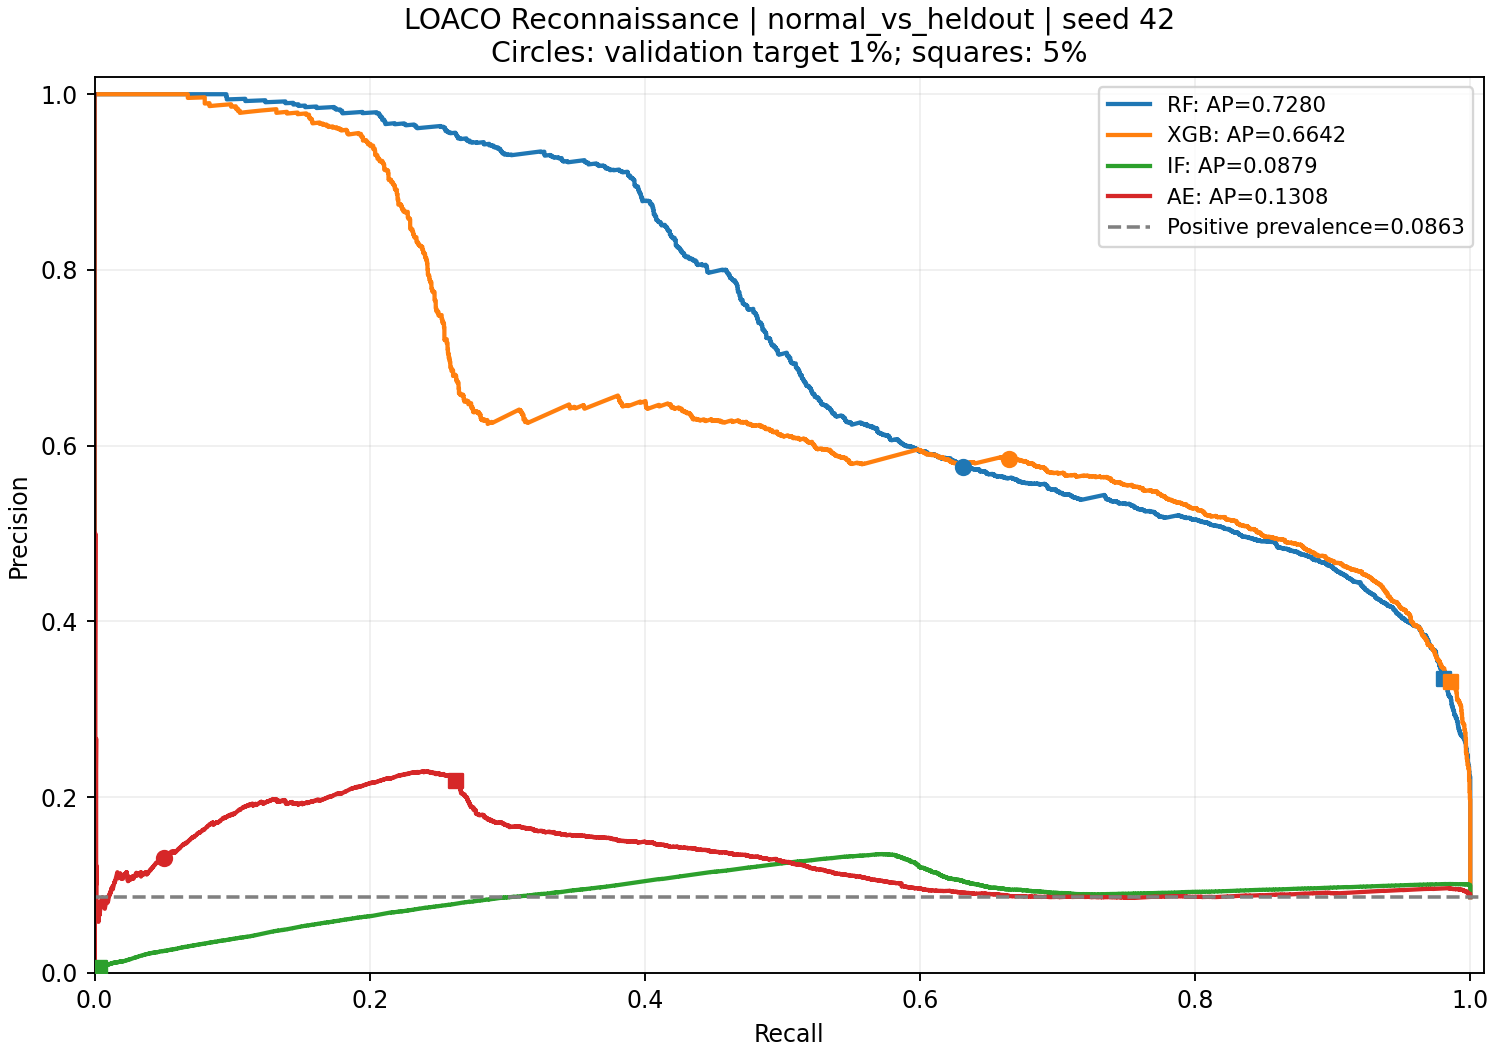
\includegraphics[width=.90\textwidth]{assets/dot3_20261025/PR_LR_normal_vs_heldout_S42.png}
\caption{PR ở LOACO Reconnaissance, chỉ Normal và held-out; seed 42 minh họa. Chấm/trục dùng ngưỡng validation có sẵn, không dùng đường test chọn lại ngưỡng.}
\end{figure}

\begin{figure}[H]\centering
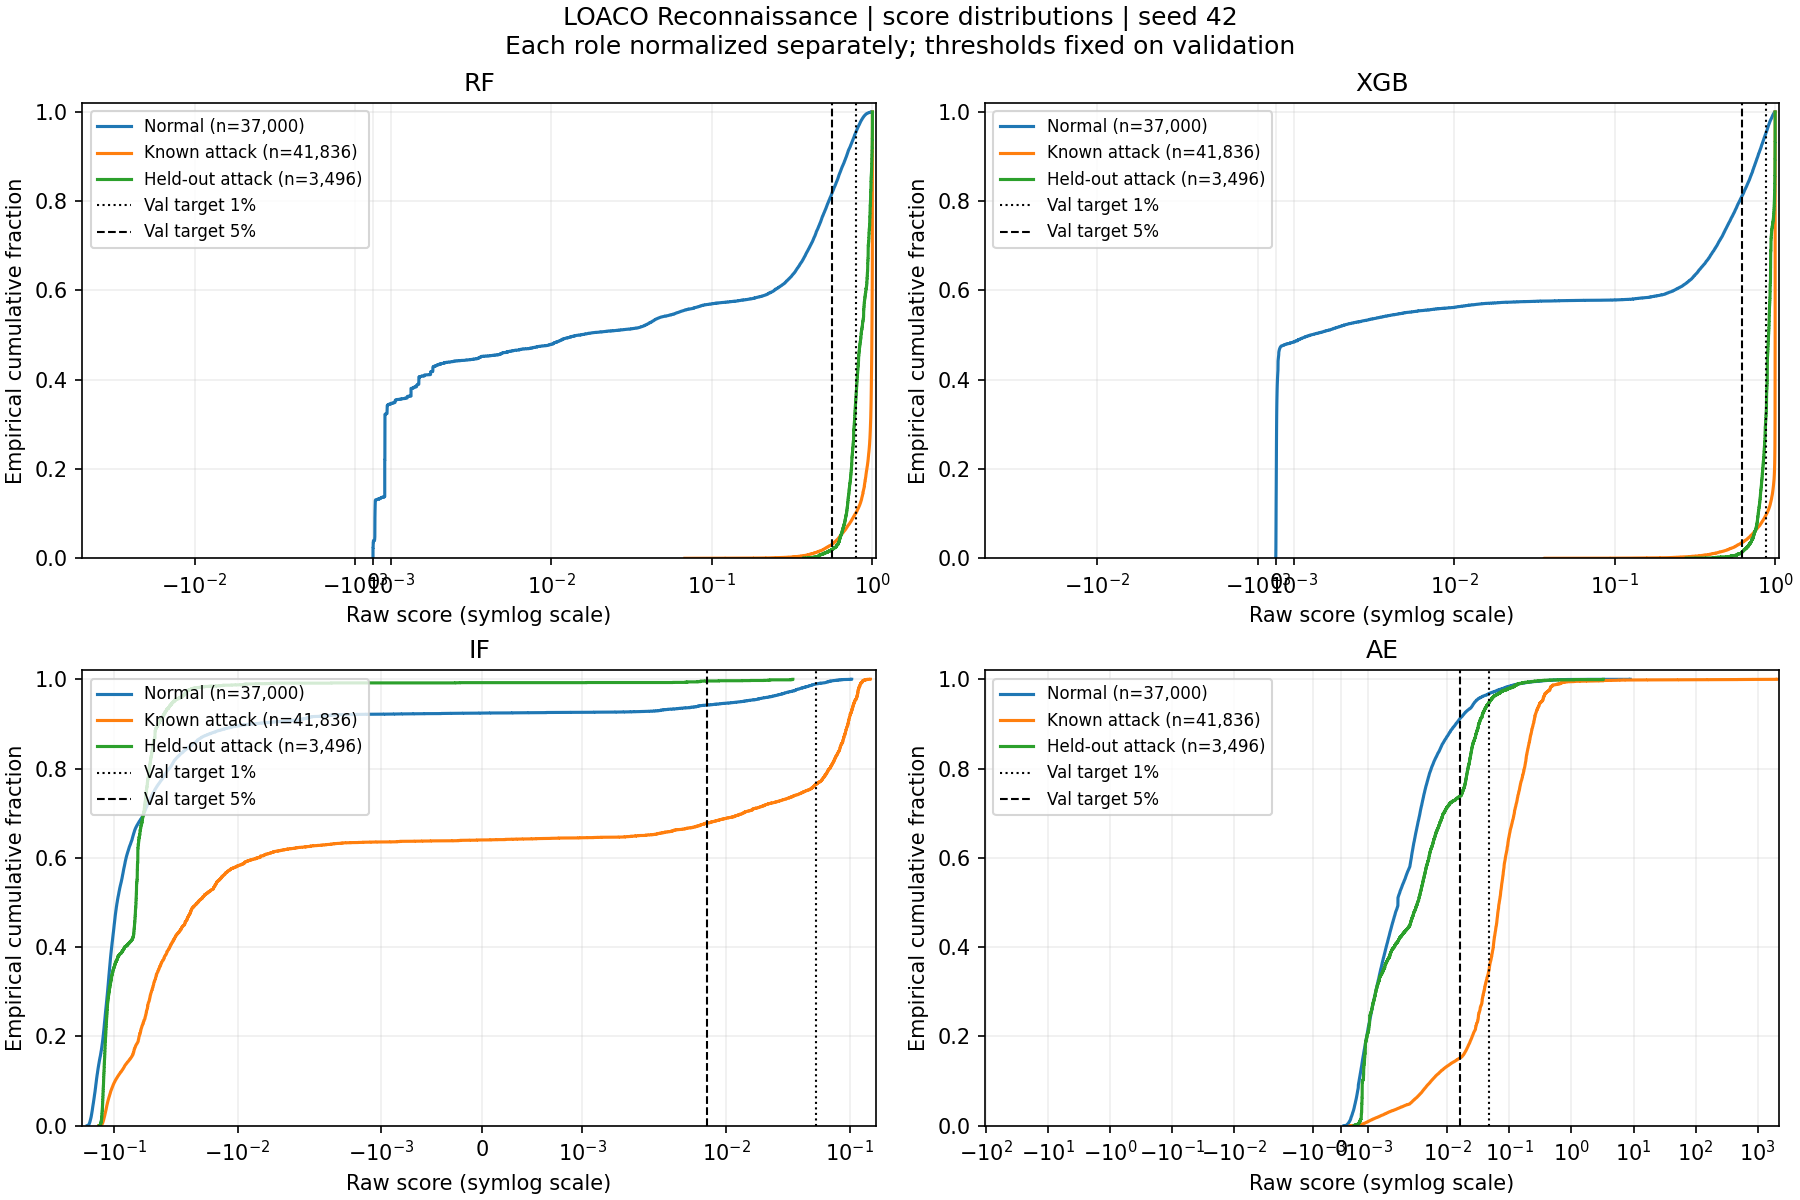
\includegraphics[width=.95\textwidth]{assets/dot3_20261025/SCORE_ECDF_LR_S42.png}
\caption{ECDF score theo Normal/known/held-out và hai threshold, LR seed 42. Score khác thang giữa các mô hình; hình mô tả mức chồng lấn, chưa chứng minh nguyên nhân lỗi.}
\end{figure}

\section{Độ nhạy mô tả theo feature overlap}
Đặc tả đã ghi trước khi chạy ở \path{docs/management/DAC_TA_OVERLAP_DOT_03_20261025.md}. Mẫu test thuộc nhóm \textit{matched} khi 42 feature raw bằng một vector trong tập model thực sự được fit, không dùng id/label/attack\_cat làm key. Khử key trùng phía fit để mỗi record test chỉ đếm một lần. Nhóm còn lại là \textit{unmatched}. Match không phải cùng sự kiện mạng hoặc cùng nhãn.

Với từng seed/scenario, pipeline tái dựng chia development bằng stratify attack\_cat, loại held-out trước chia. RF/XGB fit toàn development train; IF/AE chỉ fit Normal. Phạm vi fit được kiểm bằng fingerprint cấu hình/dữ liệu, ID partition trong audit lịch sử, số dòng và mean/variance scaler trong bundle đã lưu. Đây là tái dựng có kiểm chứng, không phải nhật ký từng row fit được ghi trực tiếp khi huấn luyện.

Hai nhóm giữ nguyên score, threshold và prediction. Tổng support và TP/FP/TN/FN hai nhóm bằng toàn test ở mỗi run/target; 1.040 metric gốc tiếp tục khớp. Khi không có mẫu số, bảng ghi --; CSV giữ NaN và số seed hợp lệ. AP của nhóm chỉ có một nhãn cũng ghi thiếu, không diễn giải là AP=0. RF/XGB dùng cùng phạm vi fit, IF/AE cùng Normal-only; nhóm matched khác nhau giữa hai họ và có thể khác theo seed.
\begingroup\small\setlength{\tabcolsep}{3pt}\renewcommand{\arraystretch}{1.18}
\begin{longtable}{L{1.3cm}L{2.1cm}L{3.4cm}L{3.4cm}L{3.4cm}}
\caption{Support nhóm matched theo vai trò; min--max qua năm seed}\\
\toprule Sc. & Phạm vi fit & Normal & Known Attack & Held-out Attack\\\midrule
\endfirsthead
\multicolumn{5}{l}{\small Bảng \thetable\ (tiếp)}\\
\toprule Sc. & Phạm vi fit & Normal & Known Attack & Held-out Attack\\\midrule
\endhead
CS & RF/XGB & 1,386--1,403 & 6,454--6,768 & 0\\
CS & IF/AE & 1,095--1,146 & 15--22 & 0\\
LR & RF/XGB & 1,386--1,403 & 5,358--5,661 & 230--247\\
LR & IF/AE & 1,095--1,146 & 15--22 & 0\\
LD & RF/XGB & 1,383--1,413 & 4,734--4,852 & 1,751--1,882\\
LD & IF/AE & 1,105--1,141 & 16--21 & 0\\
LE & RF/XGB & 1,385--1,411 & 4,857--5,055 & 1,583--1,700\\
LE & IF/AE & 1,107--1,146 & 16--21 & 0\\
\bottomrule\end{longtable}\endgroup

\begingroup\small\setlength{\tabcolsep}{3pt}\renewcommand{\arraystretch}{1.18}
\begin{longtable}{L{0.65cm}L{1.25cm}L{1.45cm}L{2.35cm}L{2.4cm}L{2.45cm}L{2.45cm}}
\caption{Nhóm trùng/không trùng với tập fit; target validation 5\%; chỉ số theo \%, std theo điểm phần trăm}\\
\toprule Sc. & Model & Nhóm & Support min--max & FPR & Recall Attack & UADR\\\midrule
\endfirsthead
\multicolumn{7}{l}{\small Bảng \thetable\ (tiếp)}\\
\toprule Sc. & Model & Nhóm & Support min--max & FPR & Recall Attack & UADR\\\midrule
\endhead
CS & RF & Trùng & 7,843--8,154 & $22.55\pm0.72$ & $99.77\pm0.02$ & --\\
CS & RF & Không trùng & 74,178--74,489 & $18.41\pm0.35$ & $96.69\pm0.08$ & --\\
CS & XGB & Trùng & 7,843--8,154 & $29.41\pm0.98$ & $99.83\pm0.02$ & --\\
CS & XGB & Không trùng & 74,178--74,489 & $18.29\pm0.44$ & $96.41\pm0.15$ & --\\
CS & IF & Trùng & 1,117--1,167 & $1.92\pm1.64$ & $41.89\pm5.57$ & --\\
CS & IF & Không trùng & 81,165--81,215 & $6.28\pm0.41$ & $31.44\pm2.92$ & --\\
CS & AE & Trùng & 1,117--1,167 & $1.19\pm0.07$ & $0.00\pm0.00$ & --\\
CS & AE & Không trùng & 81,165--81,215 & $9.41\pm0.41$ & $79.43\pm1.36$ & --\\
LR & RF & Trùng & 6,978--7,294 & $23.72\pm1.18$ & $99.73\pm0.03$ & $100.00\pm0.00$\\
LR & RF & Không trùng & 75,038--75,354 & $18.38\pm0.26$ & $96.60\pm0.14$ & $97.56\pm0.32$\\
LR & XGB & Trùng & 6,978--7,294 & $29.47\pm0.73$ & $99.81\pm0.02$ & $99.84\pm0.23$\\
LR & XGB & Không trùng & 75,038--75,354 & $18.34\pm0.51$ & $96.18\pm0.20$ & $97.93\pm0.92$\\
LR & IF & Trùng & 1,117--1,167 & $4.00\pm6.94$ & $38.56\pm4.83$ & --\\
LR & IF & Không trùng & 81,165--81,215 & $6.27\pm0.42$ & $31.92\pm3.03$ & $0.66\pm0.26$\\
LR & AE & Trùng & 1,117--1,167 & $1.19\pm0.07$ & $0.00\pm0.00$ & --\\
LR & AE & Không trùng & 81,165--81,215 & $9.32\pm0.45$ & $79.65\pm1.42$ & $23.82\pm3.75$\\
LD & RF & Trùng & 7,898--8,126 & $24.05\pm0.46$ & $99.78\pm0.02$ & $100.00\pm0.00$\\
LD & RF & Không trùng & 74,206--74,434 & $18.54\pm0.35$ & $96.63\pm0.20$ & $99.66\pm0.06$\\
LD & XGB & Trùng & 7,898--8,126 & $29.20\pm0.60$ & $99.85\pm0.02$ & $100.00\pm0.00$\\
LD & XGB & Không trùng & 74,206--74,434 & $17.98\pm0.58$ & $96.28\pm0.19$ & $98.78\pm0.33$\\
LD & IF & Trùng & 1,121--1,158 & $5.38\pm7.01$ & $41.59\pm5.28$ & --\\
LD & IF & Không trùng & 81,174--81,211 & $6.13\pm0.33$ & $30.44\pm2.33$ & $4.21\pm0.99$\\
LD & AE & Trùng & 1,121--1,158 & $1.17\pm0.09$ & $0.00\pm0.00$ & --\\
LD & AE & Không trùng & 81,174--81,211 & $9.35\pm0.40$ & $79.80\pm0.72$ & $88.38\pm1.12$\\
LE & RF & Trùng & 7,829--8,163 & $25.89\pm1.56$ & $99.78\pm0.01$ & $100.00\pm0.00$\\
LE & RF & Không trùng & 74,169--74,503 & $18.02\pm0.81$ & $95.67\pm0.42$ & $96.54\pm0.67$\\
LE & XGB & Trùng & 7,829--8,163 & $29.61\pm1.38$ & $99.85\pm0.02$ & $100.00\pm0.00$\\
LE & XGB & Không trùng & 74,169--74,503 & $18.28\pm0.58$ & $95.43\pm0.27$ & $96.56\pm0.32$\\
LE & IF & Trùng & 1,123--1,166 & $3.93\pm6.74$ & $37.54\pm10.97$ & --\\
LE & IF & Không trùng & 81,166--81,209 & $6.33\pm0.48$ & $30.02\pm0.63$ & $5.29\pm0.96$\\
LE & AE & Trùng & 1,123--1,166 & $1.18\pm0.10$ & $0.00\pm0.00$ & --\\
LE & AE & Không trùng & 81,166--81,209 & $9.25\pm0.39$ & $79.32\pm1.19$ & $80.69\pm2.90$\\
\bottomrule\end{longtable}\endgroup


\begin{figure}[H]\centering
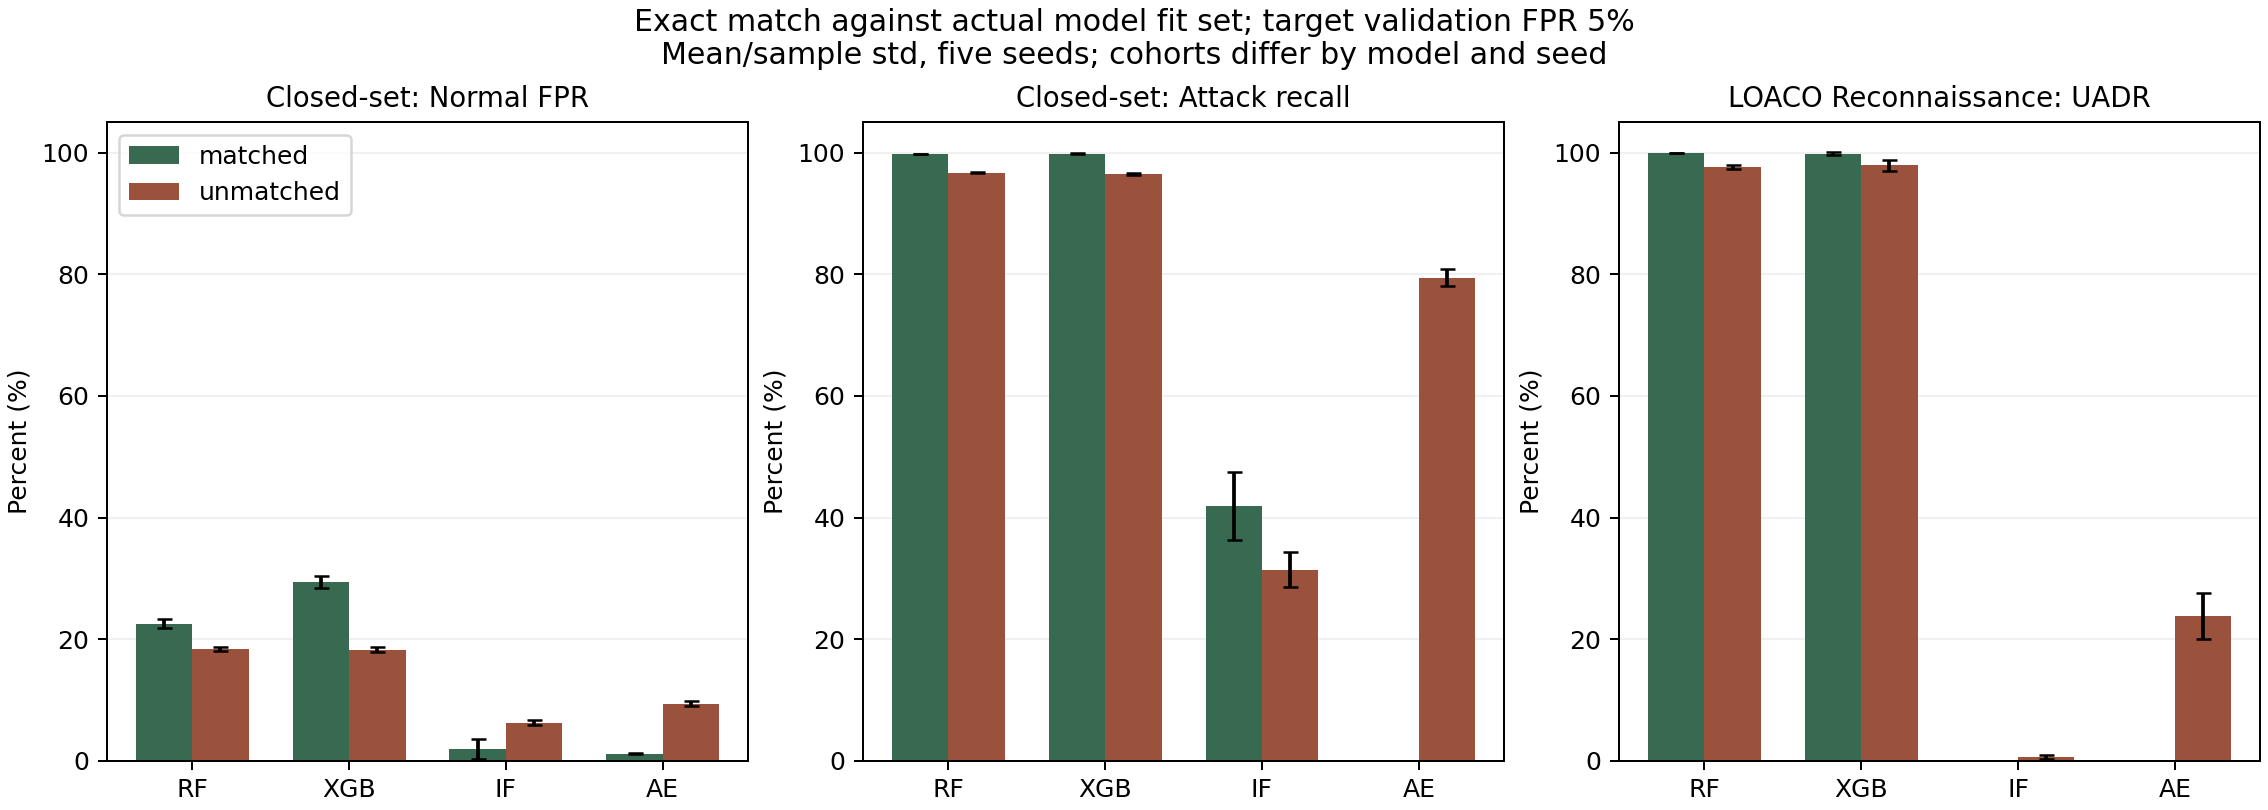
\includegraphics[width=\textwidth]{assets/dot3_20261025/OVERLAP_SLICES.png}
\caption{Ba lát cắt tại target validation 5\%; mean/sample std qua năm seed. IF/AE không có held-out matched nên UADR matched không xác định, không phải 0. Nhóm thay đổi theo model/seed; xem support trước khi so sánh.}
\end{figure}


Ví dụ LR/RF, target validation 5\%: nhóm held-out unmatched có 3.249--3.266 mẫu qua năm seed, UADR $97.56\%\pm0.32$ điểm phần trăm. Nhóm matched có 230--247 held-out. Kết quả cao còn hiện diện ngoài exact feature match; tuy nhiên không loại trừ các tương đồng khác của official split hoặc chứng minh tác động nhân quả. IF/AE không có held-out matched trong ba LOACO, nên UADR ở nhóm này không xác định.

\textbf{Giới hạn diễn giải:} đây là liên hệ mô tả giữa hai nhóm của test đang có, không phải thí nghiệm huấn luyện loại overlap. Nhãn, loại tấn công và độ khó có thể khác; chênh lệch metric không chứng minh overlap gây tăng/giảm hiệu quả. Không xem nhóm unmatched là test mới độc lập hoặc so trực tiếp các nhóm khác nhau để xếp hạng mô hình. Năm seed cùng dùng official test; sample std không phải khoảng tin cậy. Chưa thực hiện retrain loại trùng hay kiểm trên dữ liệu vận hành.

\section{Importance của feature: gợi ý đọc, chưa phải nguyên nhân lỗi}
Đã trích importance trong bundle RF/XGB cho 40 run (4 scenario, 2 model, 5 seed), gom contribution của one-hot về 42 feature raw. RF dùng mean decrease in impurity; XGB dùng normalized gain. Đây là mô tả mô hình đã fit, không phải permutation importance trên test và không cho biết feature gây ra từng FP/FN. Categorical feature có thể chịu thiên lệch do số mức.
\begingroup\small\setlength{\tabcolsep}{3pt}\renewcommand{\arraystretch}{1.18}
\begin{longtable}{L{1.3cm}L{1.2cm}L{11.3cm}}
\caption{Ba feature có importance trung bình cao nhất; mô tả theo 5 seed}\\
\toprule Sc. & Model & Ba feature đứng đầu (importance mean)\\\midrule
\endfirsthead
\multicolumn{3}{l}{\small Bảng \thetable\ (tiếp)}\\
\toprule Sc. & Model & Ba feature đứng đầu (importance mean)\\\midrule
\endhead
CS & RF & sttl (0.097); ct\_state\_ttl (0.076); sload (0.052)\\
CS & XGB & sttl (0.603); proto (0.094); ct\_state\_ttl (0.090)\\
LR & RF & sttl (0.096); ct\_state\_ttl (0.075); sload (0.052)\\
LR & XGB & sttl (0.564); proto (0.102); ct\_state\_ttl (0.090)\\
\bottomrule\end{longtable}\endgroup


\begin{figure}[H]\centering
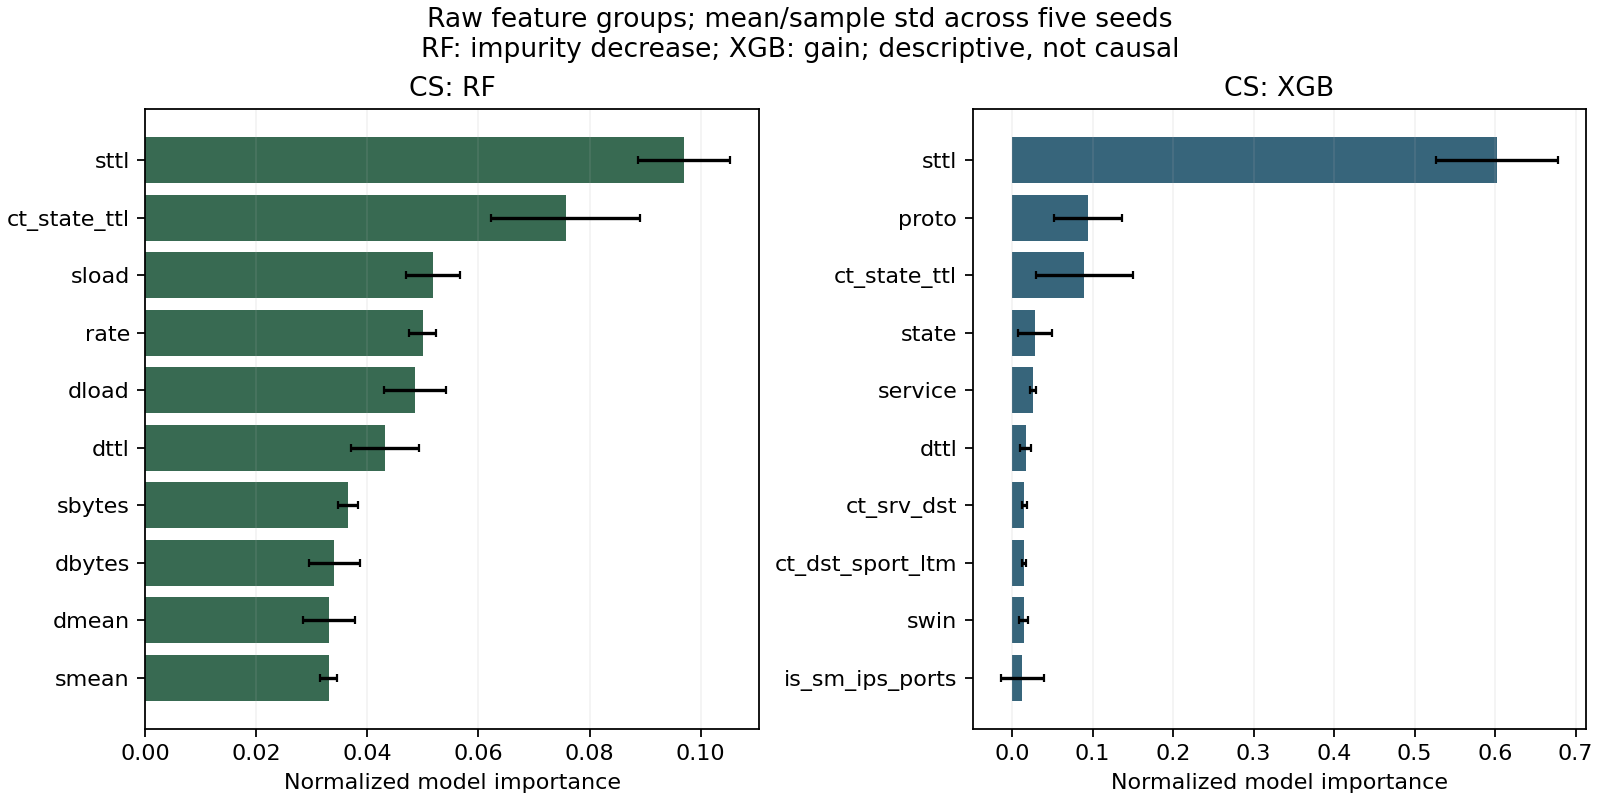
\includegraphics[width=.92\textwidth]{assets/dot3_20261025/FEATURES_CS.png}
\caption{Mười feature đứng đầu ở closed-set; mean/sample std qua năm seed. RF và XGB dùng định nghĩa importance khác nhau.}
\end{figure}
\begin{figure}[H]\centering
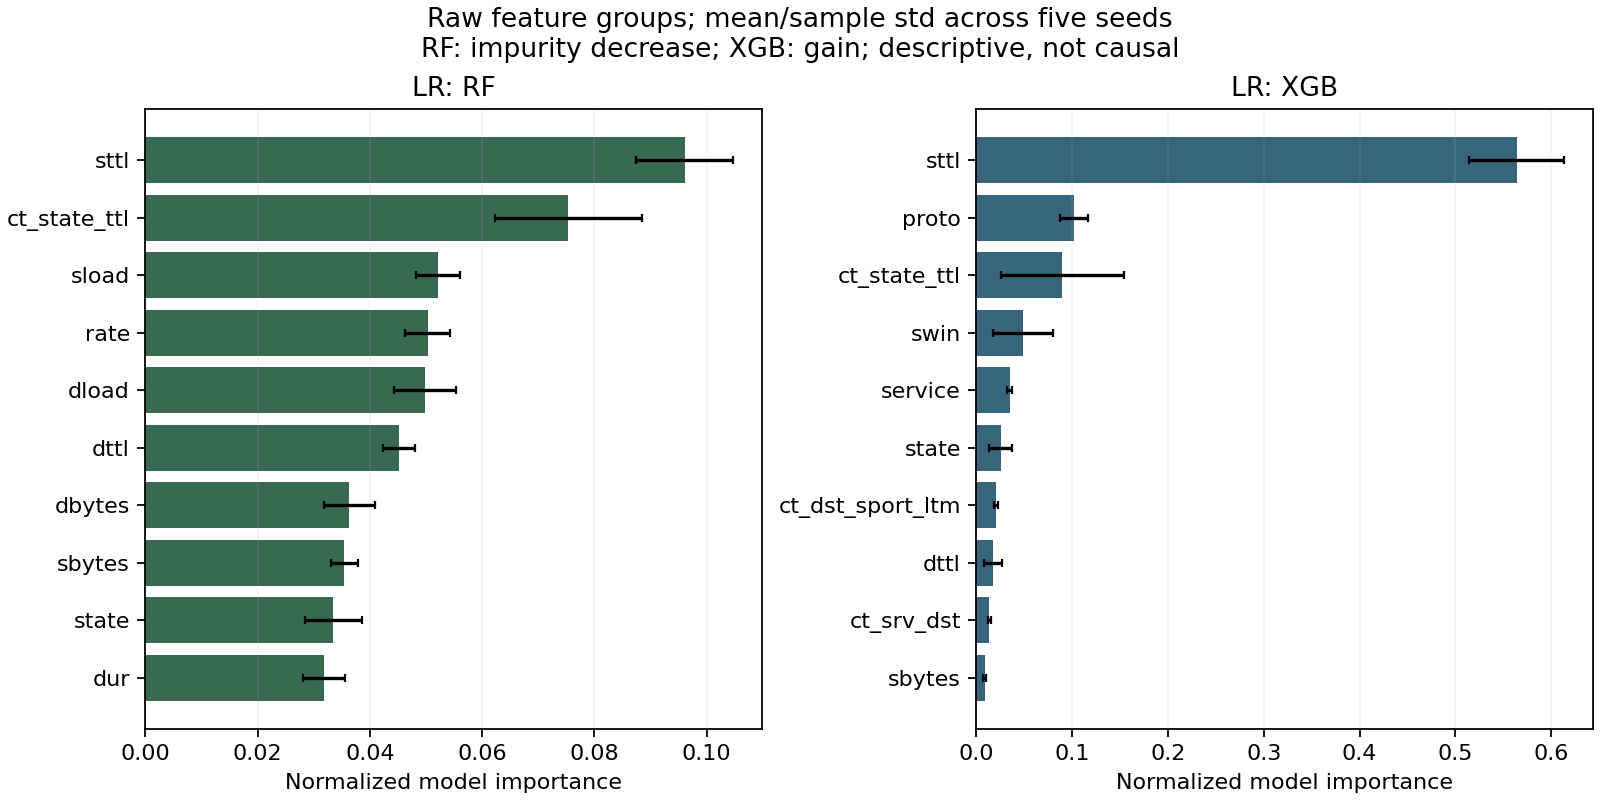
\includegraphics[width=.92\textwidth]{assets/dot3_20261025/FEATURES_LR.png}
\caption{Mười feature đứng đầu ở LOACO Reconnaissance; mô tả feature quan trọng trong mô hình, chưa là giải thích nhân quả.}
\end{figure}


\section{Đọc trade-off, ma trận lỗi và độ ổn định}
Phần này hoàn tất bộ hình dự kiến từ prediction đã khóa. Hai target 1\%/5\% do validation quyết định; trục FPR trong hình trade-off là FPR quan sát trên test. Mean/sample std dùng năm seed trên cùng official test, không phải khoảng tin cậy hoặc bằng chứng tổng quát ra hệ thống vận hành. CS không có held-out nên không vẽ UADR CS. Ma trận dùng seed 42 đã định trước, không chọn seed có kết quả đẹp.

\begin{figure}[H]\centering
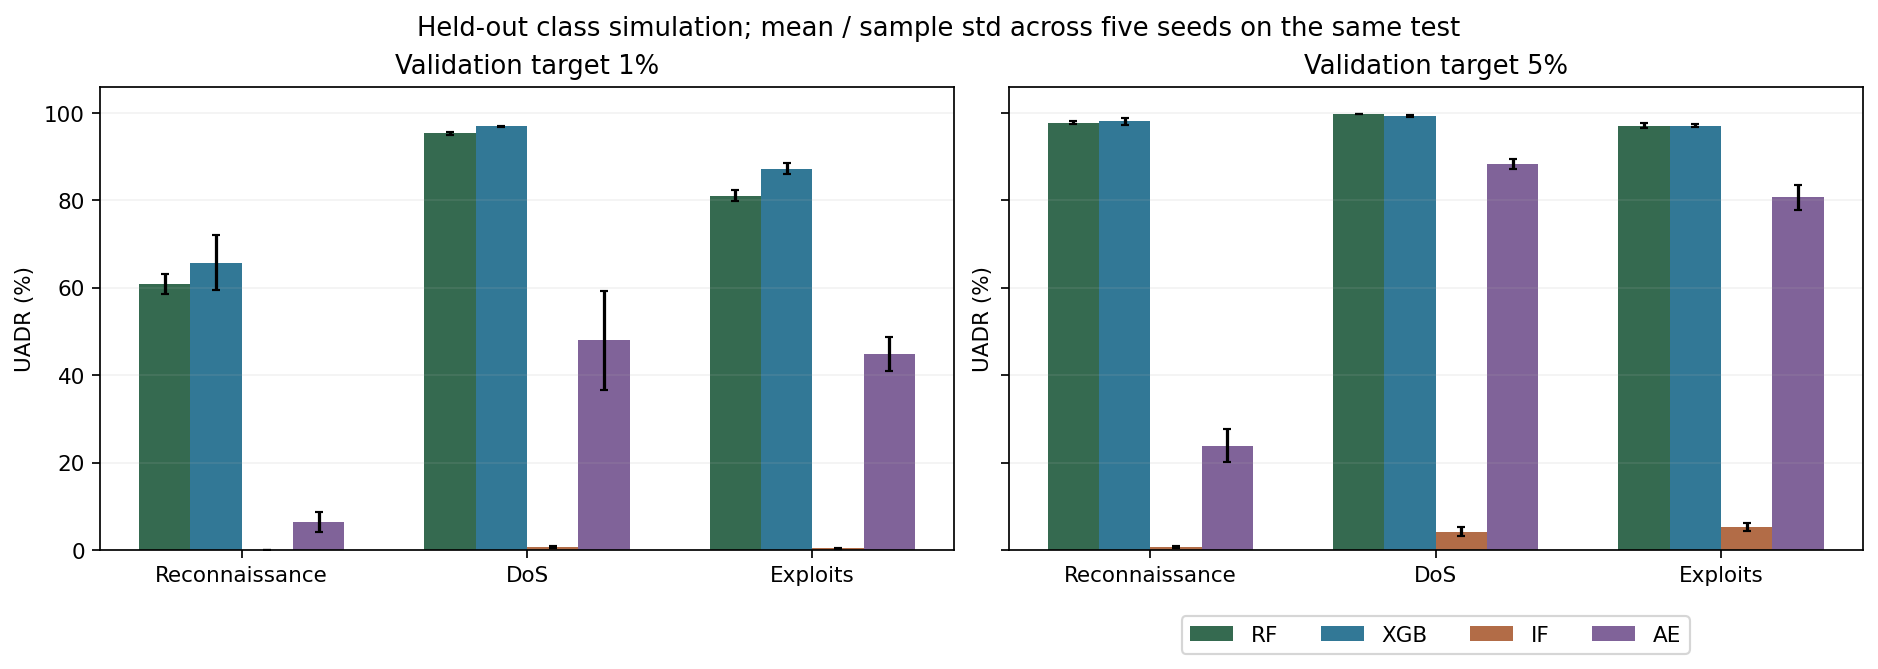
\includegraphics[width=.98\textwidth]{assets/final_diagnostics/UADR_BOTH_TARGETS.png}
\caption{UADR theo ba lớp held-out ở hai target validation; mean/sample std qua năm seed, mô phỏng giấu lớp.}\end{figure}

\begin{figure}[H]\centering
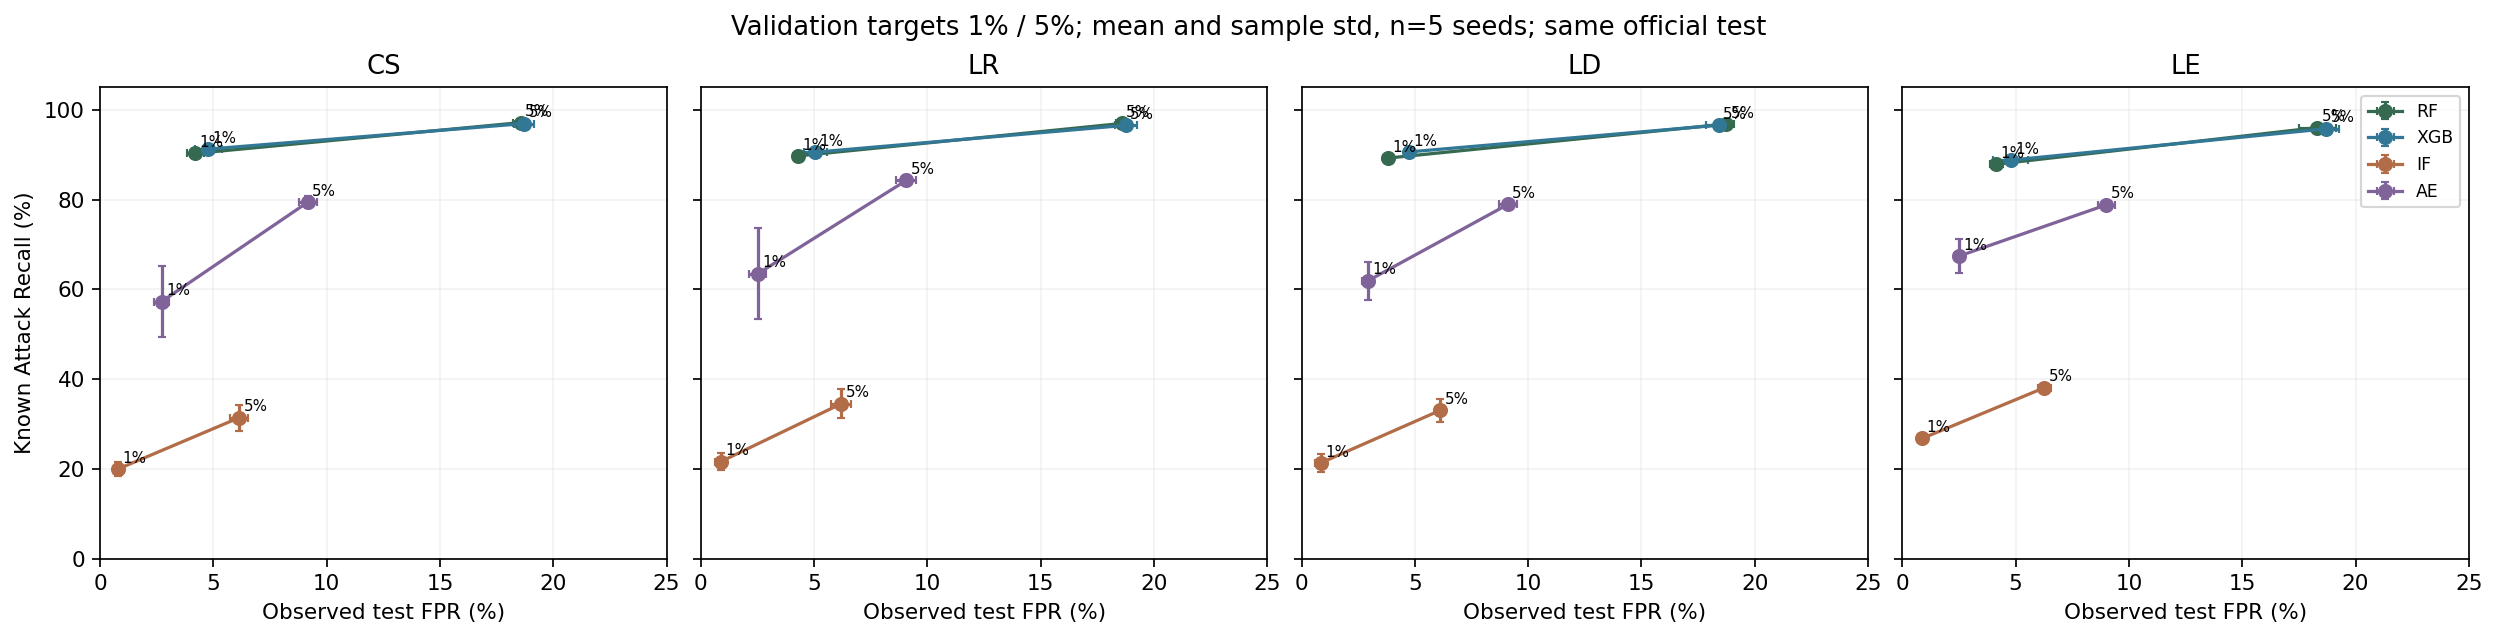
\includegraphics[width=.98\textwidth]{assets/final_diagnostics/TRADEOFF_KNOWN_RECALL.png}
\caption{Known Attack Recall theo FPR test quan sát; hai điểm là target validation 1\%/5\%, mean/sample std năm seed.}\end{figure}

\begin{figure}[H]\centering
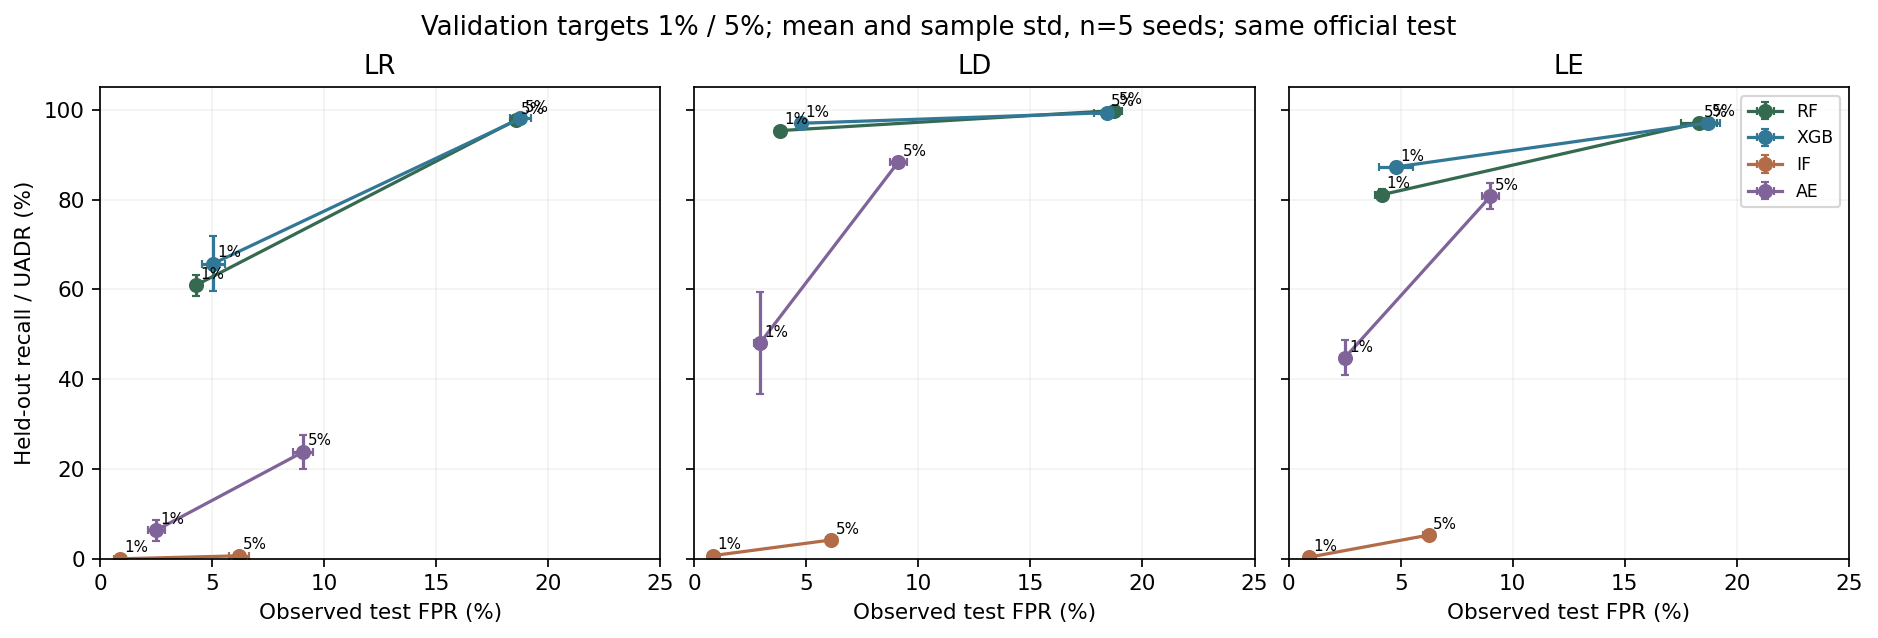
\includegraphics[width=.98\textwidth]{assets/final_diagnostics/TRADEOFF_UADR.png}
\caption{UADR theo FPR test quan sát; ba LOACO, mean/sample std năm seed. Đọc đồng thời khả năng bắt held-out và báo nhầm.}\end{figure}

\begin{figure}[H]\centering
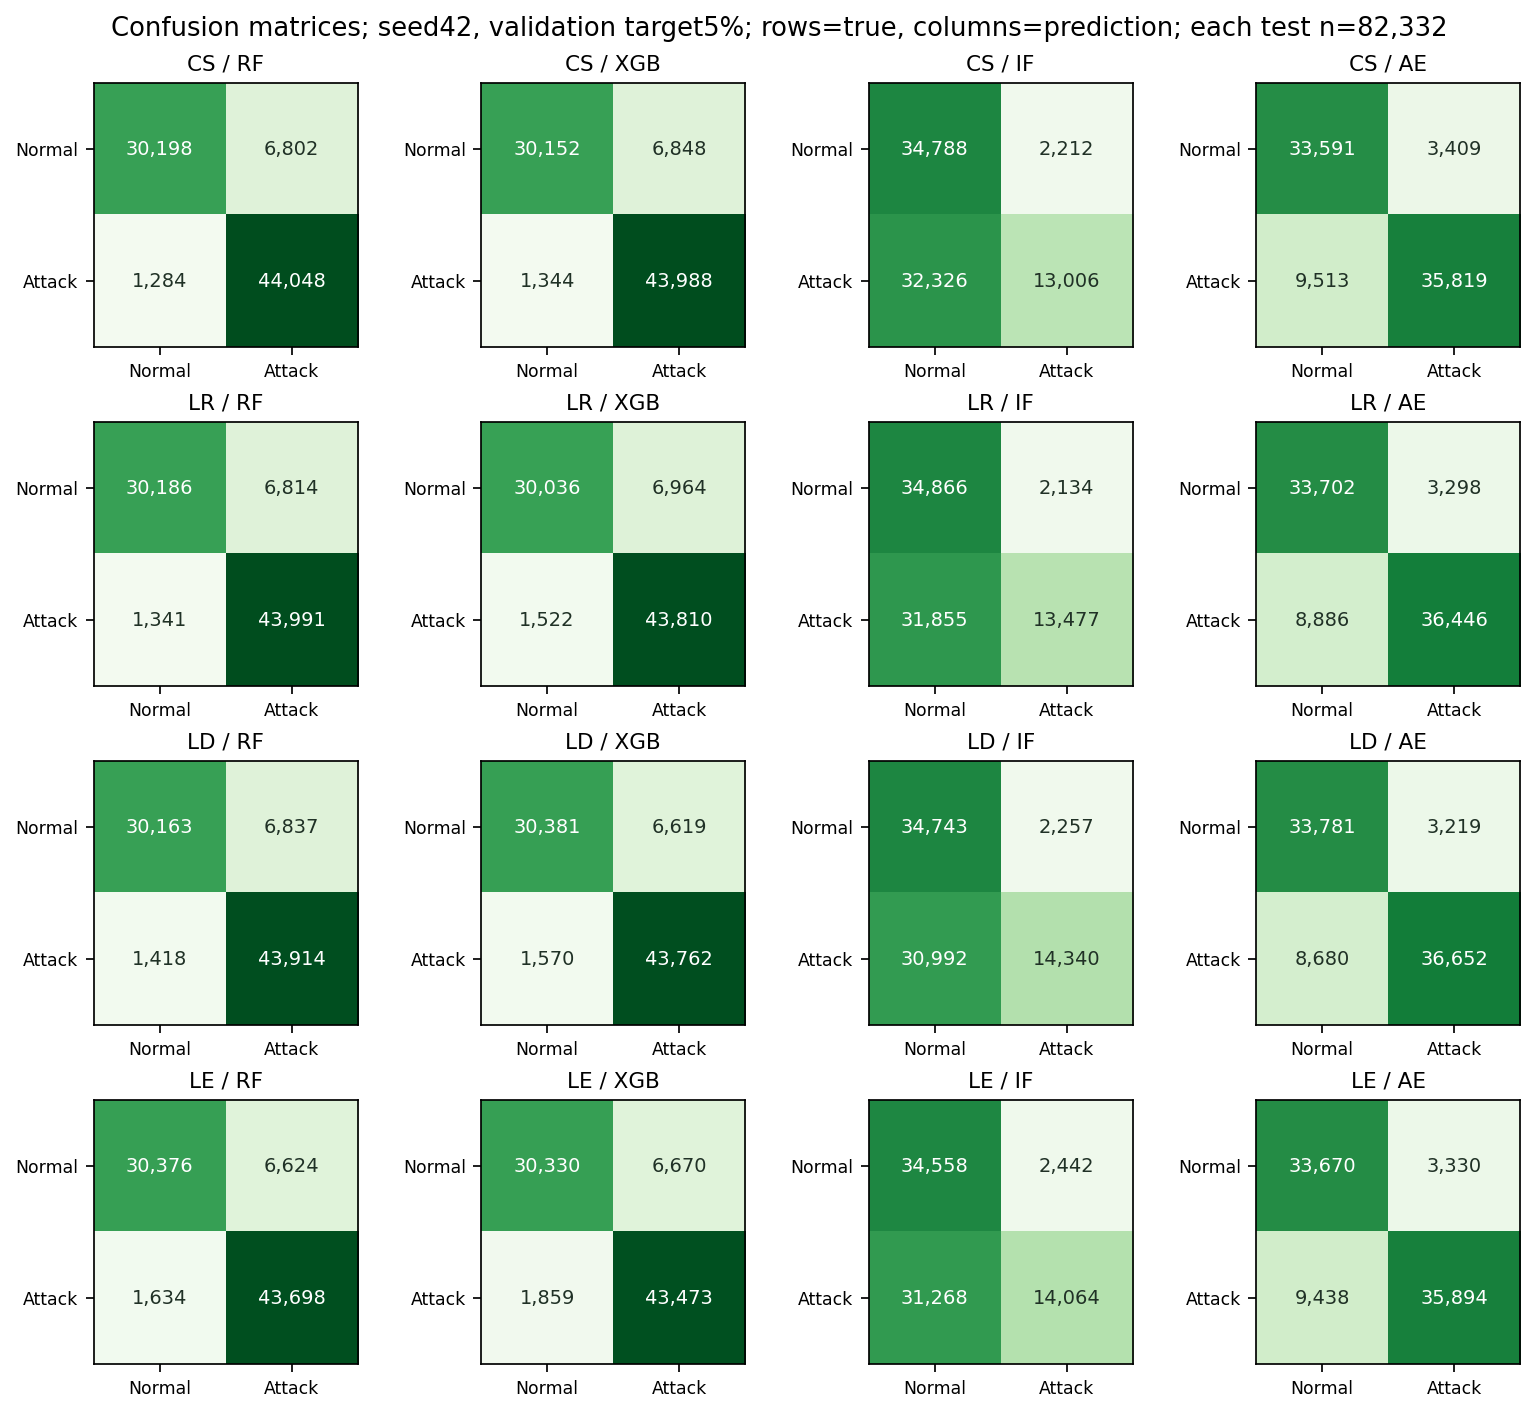
\includegraphics[width=.94\textwidth]{assets/final_diagnostics/CONFUSION_ALL_SCENARIOS_S42.png}
\caption{Ma trận nhầm lẫn cho CS và ba LOACO, bốn model, seed 42, target validation 5\%. Hàng là nhãn thật, cột là dự đoán.}\end{figure}

\begin{figure}[H]\centering
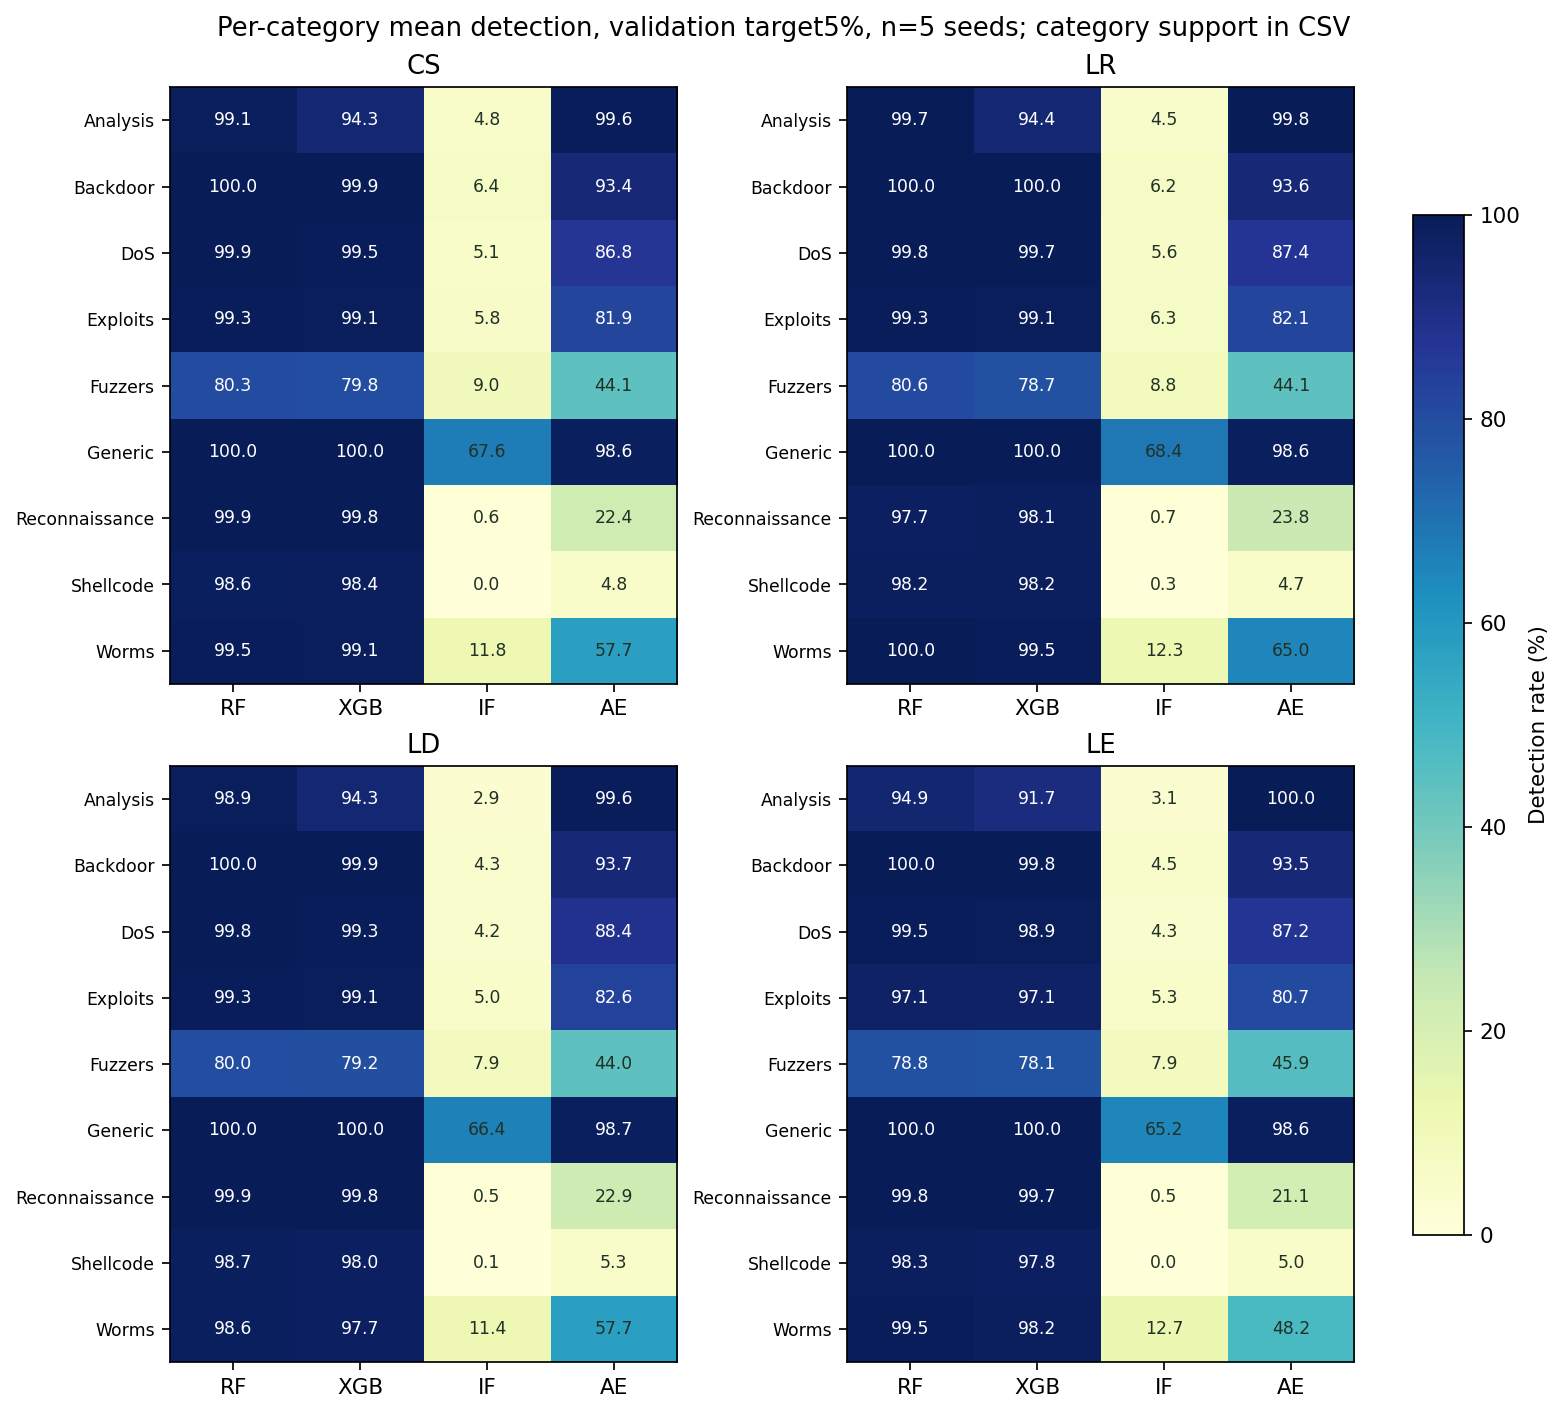
\includegraphics[width=.94\textwidth]{assets/final_diagnostics/CATEGORY_DETECTION_HEATMAP.png}
\caption{Detection rate từng attack category, target validation 5\%; mean năm seed; support đầy đủ trong CSV category.}\end{figure}

\begin{figure}[H]\centering
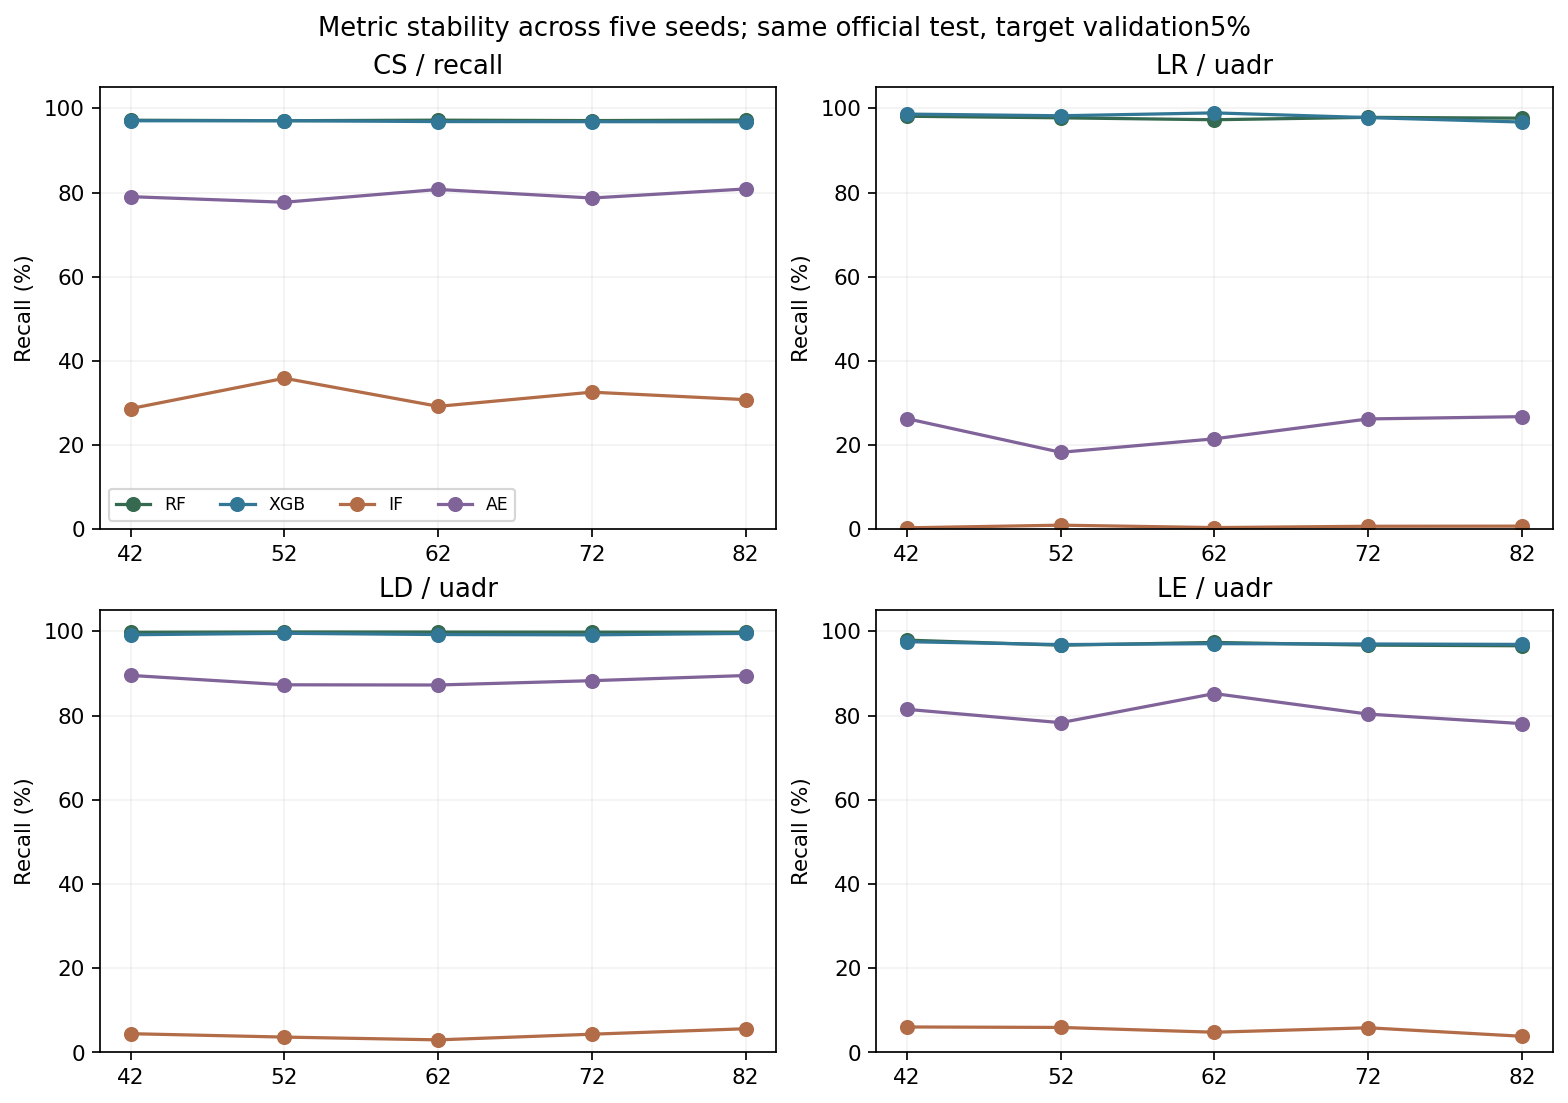
\includegraphics[width=.98\textwidth]{assets/final_diagnostics/SEED_STABILITY.png}
\caption{Độ biến thiên theo seed trên cùng test. CS dùng recall Attack; LOACO dùng UADR; target validation 5\%.}\end{figure}

\begin{figure}[H]\centering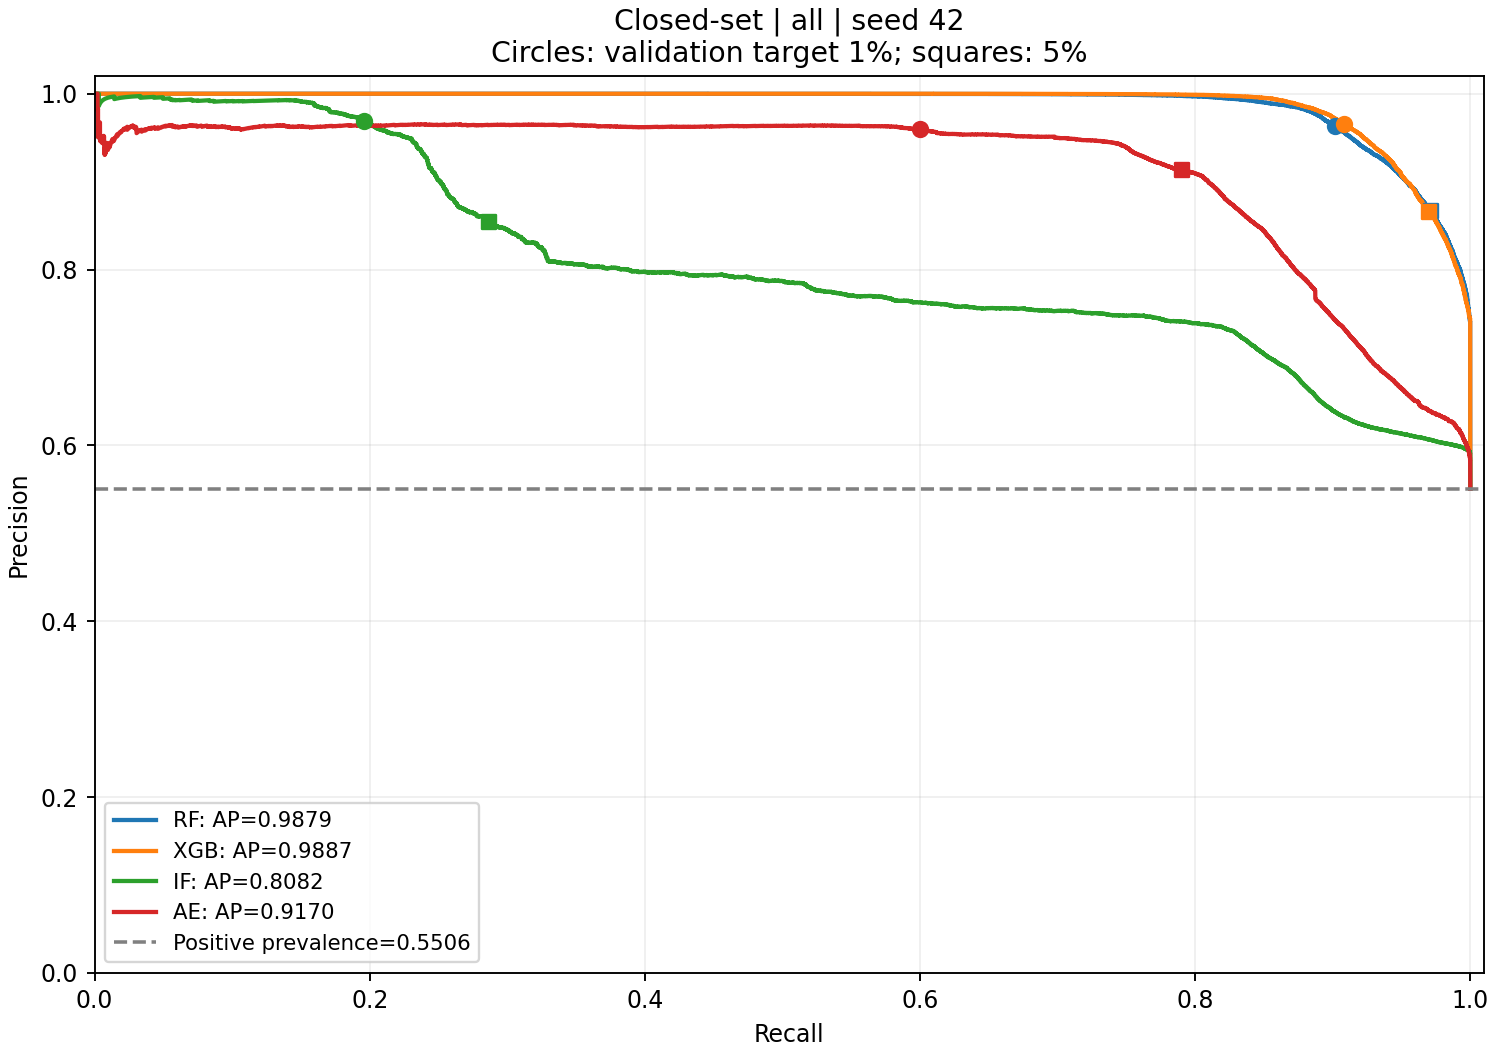
\includegraphics[width=.92\textwidth]{assets/dot3_20261025/PR_CS_all_S42.png}\caption{PR closed-set cho bốn model, seed 42; AP dùng một score mỗi record, hai target chỉ xác định điểm vận hành.}\end{figure}

\begin{figure}[H]\centering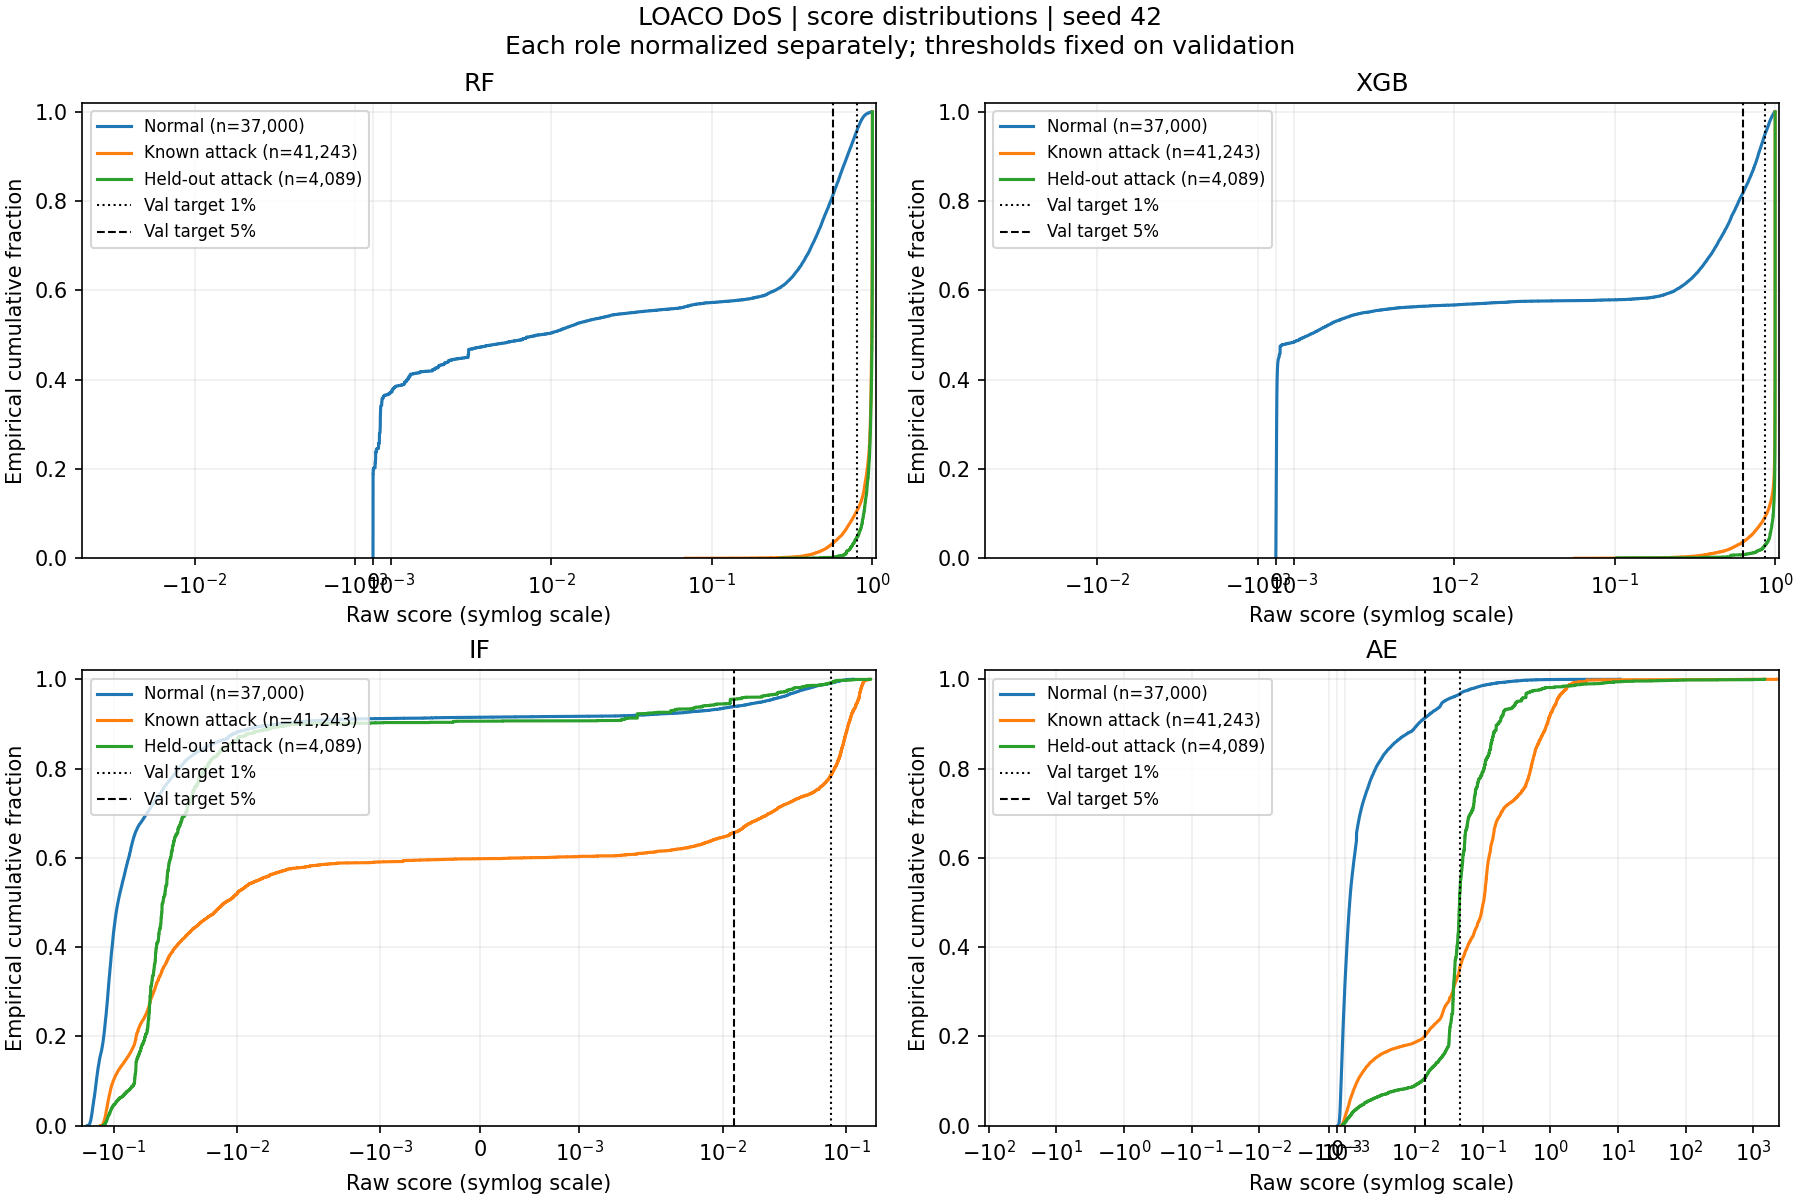
\includegraphics[width=.96\textwidth]{assets/dot3_20261025/SCORE_ECDF_LD_S42.png}\caption{ECDF score LOACO DoS, seed 42; Normal, known Attack, held-out và hai threshold validation.}\end{figure}

\begin{figure}[H]\centering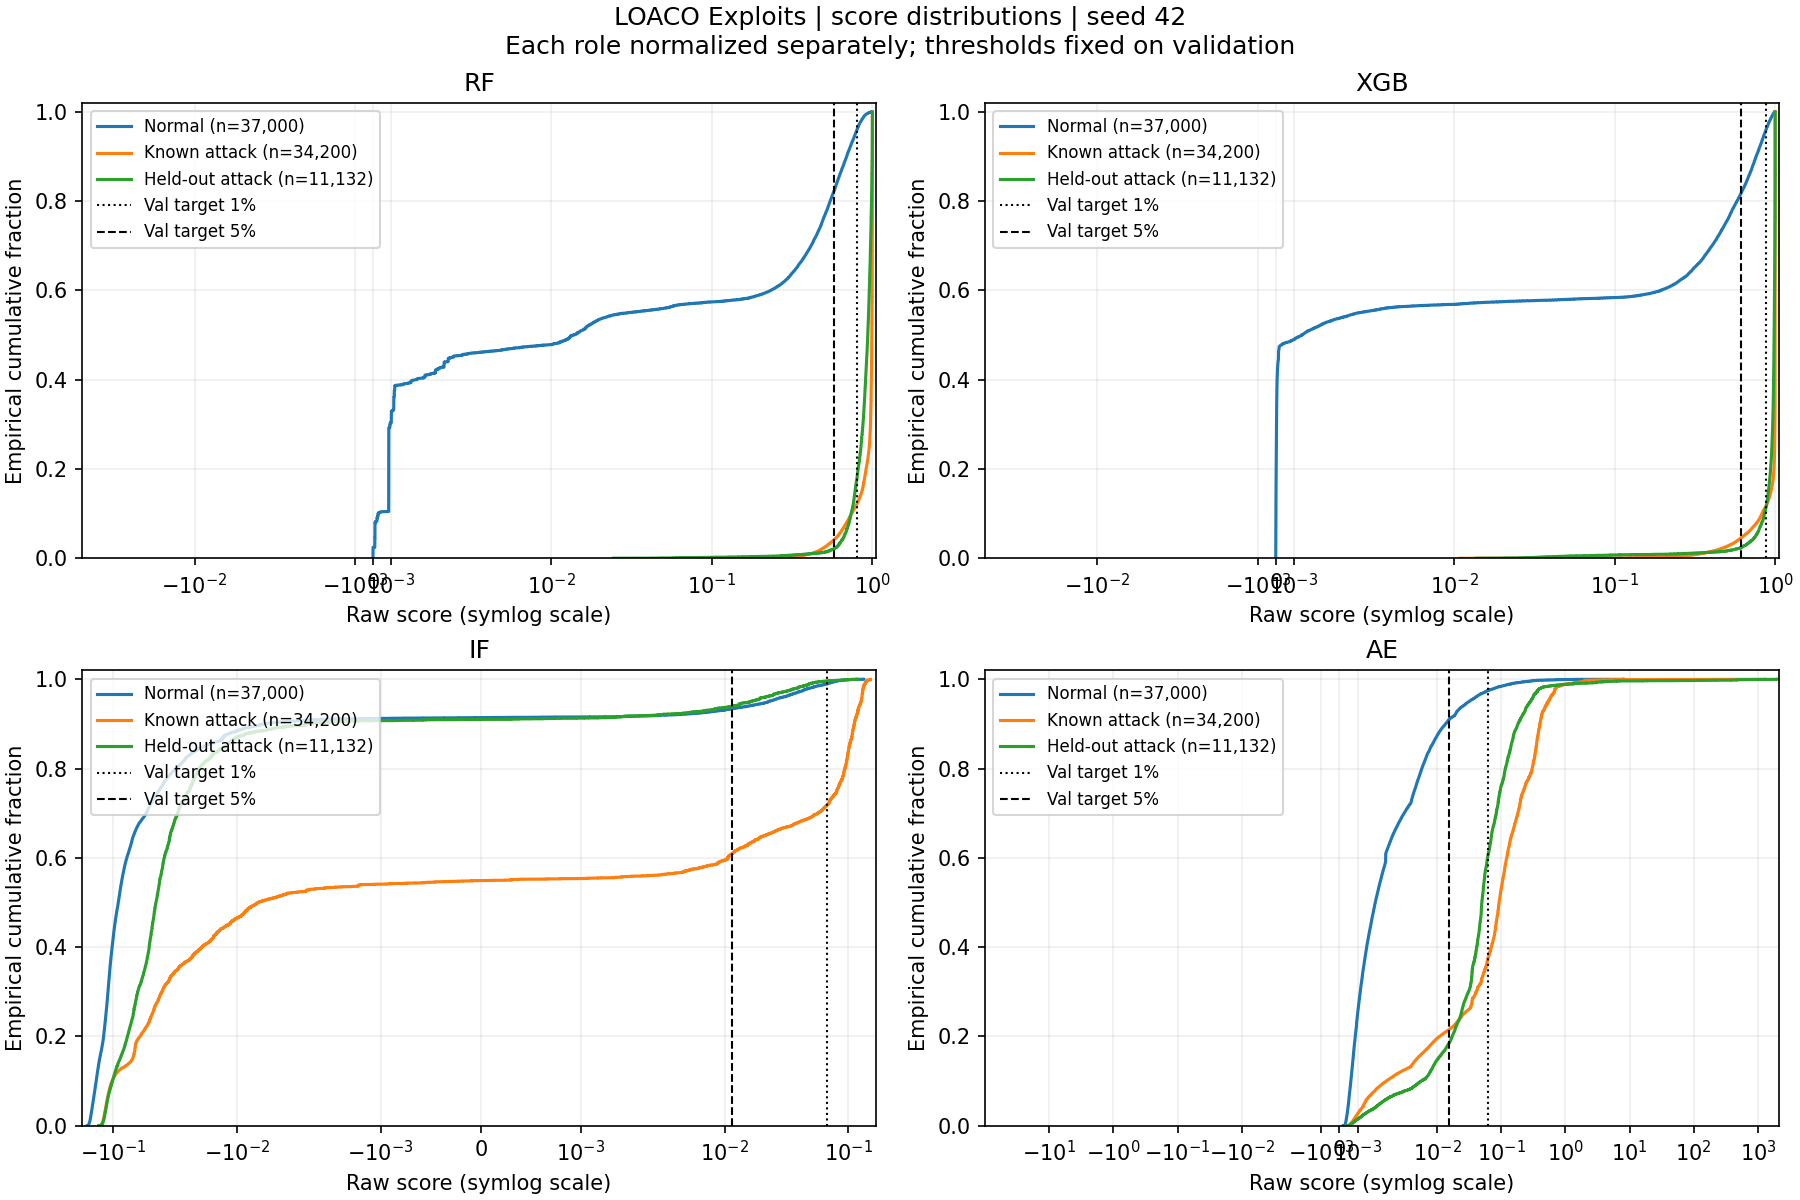
\includegraphics[width=.96\textwidth]{assets/dot3_20261025/SCORE_ECDF_LE_S42.png}\caption{ECDF score LOACO Exploits, seed 42; Normal, known Attack, held-out và hai threshold validation.}\end{figure}

\section{Lỗi theo protocol, service và state}
Đặc tả \path{docs/management/DAC_TA_CHAN_DOAN_CUOI_20261025.md} ghi quy tắc trước chạy. Ghép từng prediction về raw official test theo ID, kiểm nhãn/category/role và đủ hai target; 80 run, 13.173.120 dòng prediction và 1.040 metric gốc tiếp tục khớp. Với mỗi giá trị proto/service/state, tính support và TP/FP/TN/FN riêng theo Normal, known Attack, held-out Attack. Ở Normal, tỷ lệ lỗi là FP/support; ở Attack là FN/support. Không cộng ba chiều rồi coi là số record độc lập.

Bảng sau chọn một giá trị có tỷ lệ lỗi mean cao nhất trong mỗi chiều, model và scope, chỉ trong nhóm support ít nhất 100. Hình giữ tối đa sáu nhóm cùng quy tắc. Đây là chọn để thăm dò lỗi trong test đang có, không kiểm định giả thuyết mới, không ước lượng nhân quả, không đại diện nhóm ít mẫu bị lược khỏi hình. CSV giữ toàn bộ nhóm và cả target 1\%/5\%; support của nhóm không thay giữa seed trong cùng role/scenario.
\begingroup\small\setlength{\tabcolsep}{3pt}\renewcommand{\arraystretch}{1.18}
\begin{longtable}{L{.6cm}L{1.1cm}L{1.4cm}L{3.3cm}rL{3.4cm}}
\caption{Lát cắt lỗi thăm dò tại target validation 5\%; mean/sample std năm seed; tỷ lệ lỗi theo \%, std theo điểm phần trăm}\\
\toprule Sc. & Model & Chiều & Giá trị & Support & Tỷ lệ lỗi\\\midrule
\endfirsthead
\multicolumn{6}{l}{\small Bảng \thetable\ (tiếp)}\\
\toprule Sc. & Model & Chiều & Giá trị & Support & Tỷ lệ lỗi\\\midrule
\endhead
CS & RF & proto & udp & 8,097 & $25.89\pm0.35$\\
CS & RF & service & ftp & 758 & $32.01\pm2.25$\\
CS & RF & state & INT & 4,485 & $46.65\pm0.54$\\
CS & IF & proto & arp & 987 & $10.15\pm2.66$\\
CS & IF & service & http & 4,013 & $8.45\pm1.15$\\
CS & IF & state & REQ & 1,707 & $33.52\pm3.83$\\
LR & RF & proto & tcp & 1,865 & $3.03\pm0.06$\\
LR & RF & service & - & 2,992 & $2.63\pm0.34$\\
LR & RF & state & FIN & 1,861 & $2.99\pm0.06$\\
LR & IF & proto & udp & 1,304 & $99.95\pm0.04$\\
LR & IF & service & http & 470 & $99.53\pm0.10$\\
LR & IF & state & FIN & 1,861 & $99.88\pm0.02$\\
\bottomrule\end{longtable}\endgroup

\begin{figure}[H]\centering
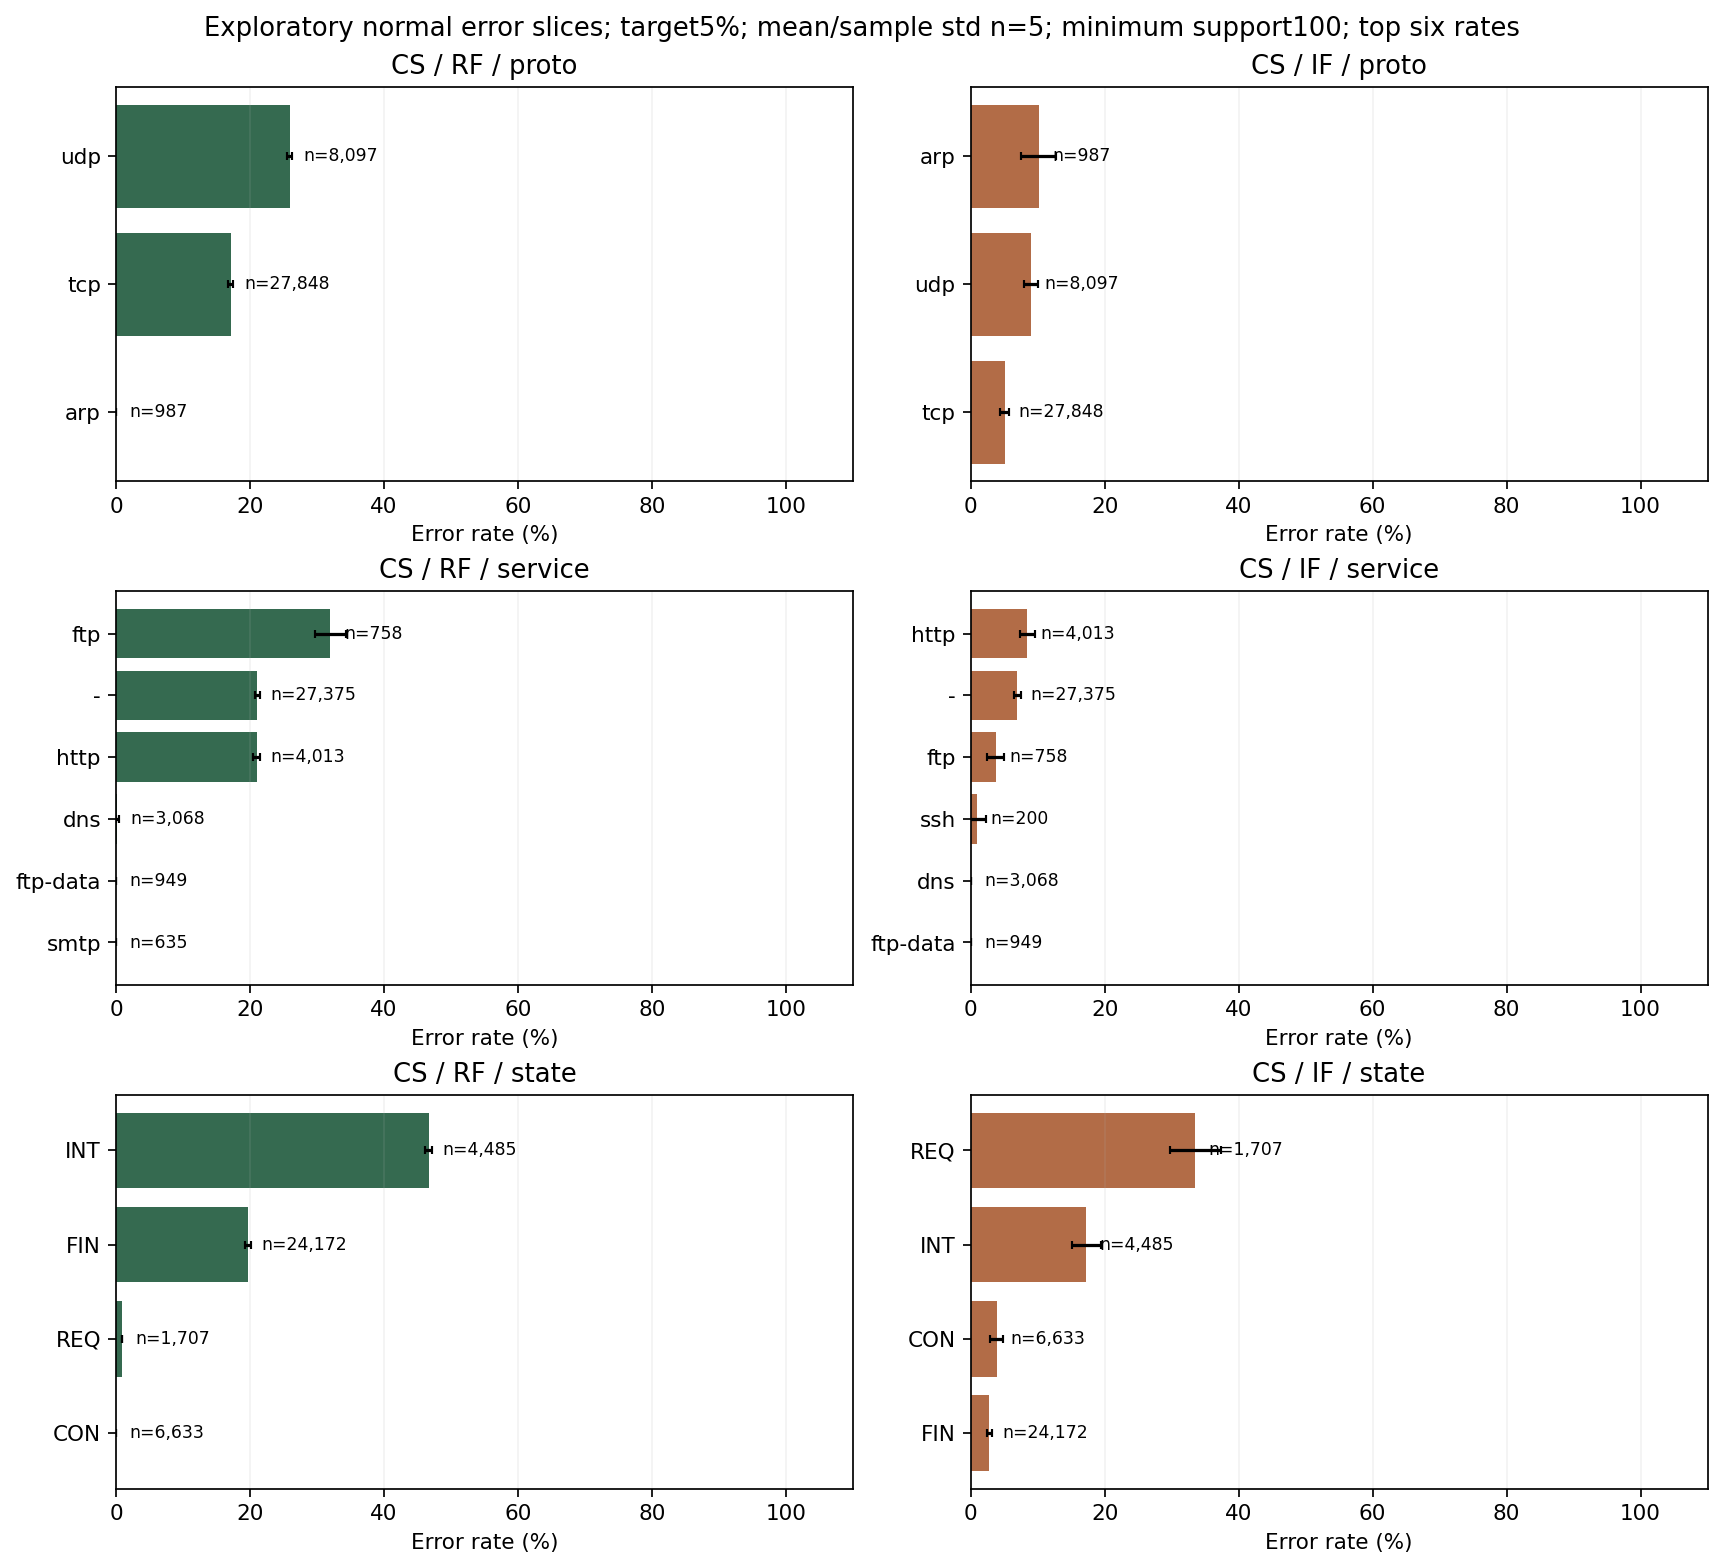
\includegraphics[width=.93\textwidth]{assets/final_diagnostics/FP_GROUPS_CS.png}
\caption{Lỗi Normal closed-set (FP), RF/IF, target validation 5\%; nhóm support tối thiểu 100, chọn tối đa sáu tỷ lệ cao nhất, mean/sample std năm seed.}\end{figure}

\begin{figure}[H]\centering
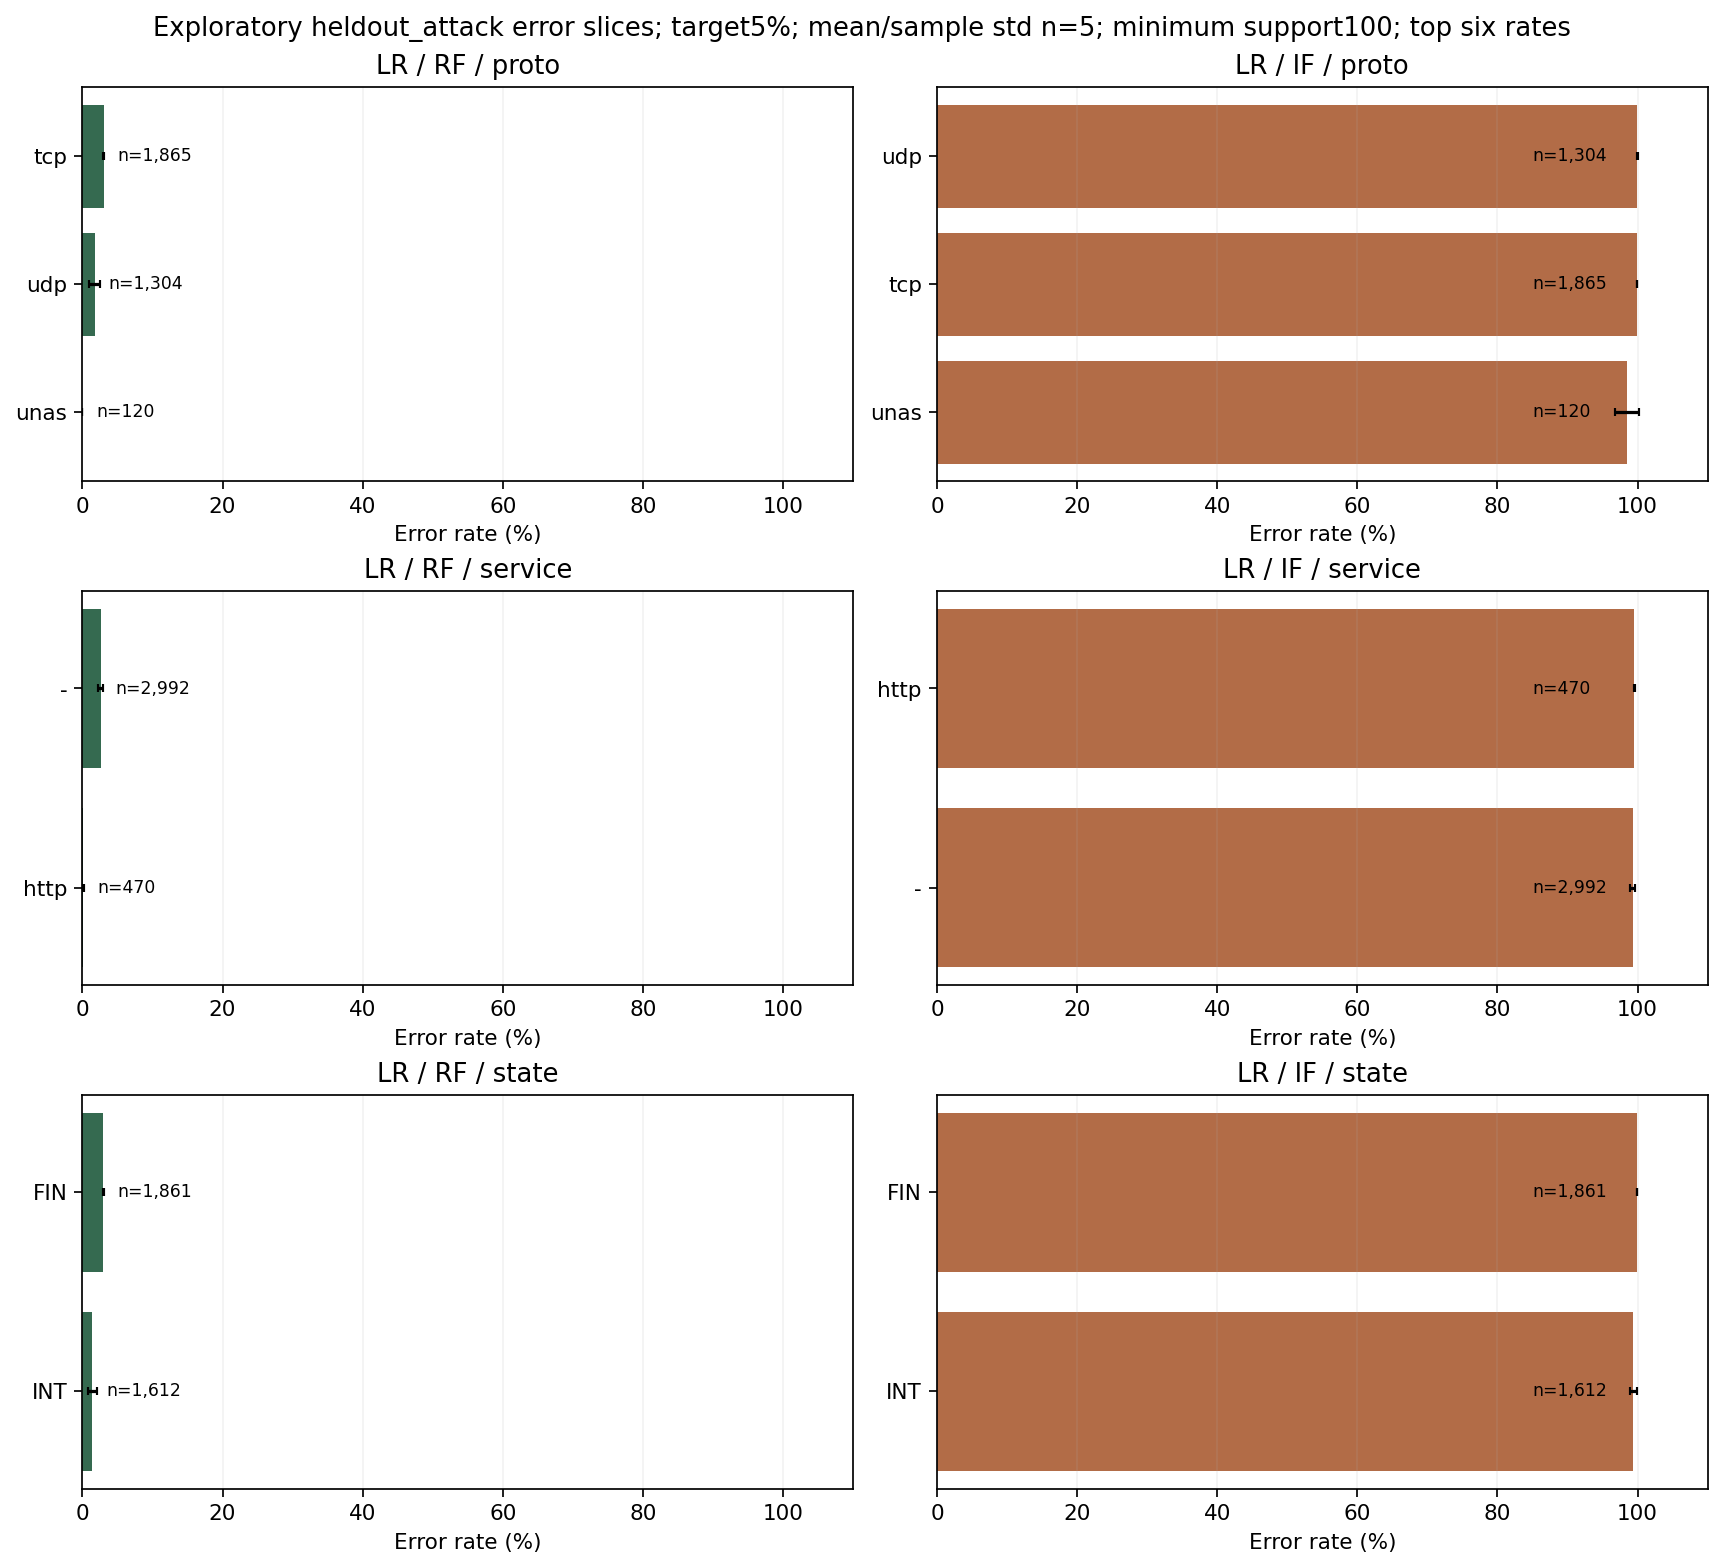
\includegraphics[width=.93\textwidth]{assets/final_diagnostics/FN_GROUPS_LR.png}
\caption{Lỗi held-out Reconnaissance (FN), RF/IF, target validation 5\%; cùng quy tắc support và chọn nhóm, mean/sample std năm seed.}\end{figure}

Tỷ lệ lỗi cao trong một service/protocol có thể đi kèm loại Attack, phân bố feature và dữ liệu gần giống nhau. Bảng này định vị chỗ cần đọc lại, không chứng minh service hoặc protocol gây lỗi. Khi trao đổi, Thu cần nêu đúng role, giá trị nhóm, support và target trước khi nói phần trăm; Anh kiểm giới hạn của phép ghép và nguồn dữ liệu.

\section{Ví dụ sát ngưỡng, lỗi lặp và bất đồng model}
Mỗi model seed 42, target và role lấy ba record có $|score-threshold|$ nhỏ nhất, hòa thì ID nhỏ trước. Bảng minh họa dưới chỉ lấy record gần nhất ở LR/RF và LR/IF cho Normal/held-out; có cả dự đoán đúng và sai, không chọn riêng trường hợp thuận lợi. dur, sttl, dbytes là feature raw để mở lại dòng gốc. Khoảng cách score chỉ đọc trong cùng model; không so khoảng cách RF với IF để nói model nào tự tin hơn. Feature importance toàn model ở phần trước không giải thích nguyên nhân từng dòng này.
\begingroup\small\setlength{\tabcolsep}{3pt}\renewcommand{\arraystretch}{1.18}
\begin{longtable}{L{1.1cm}rL{.6cm}rL{.9cm}L{1.2cm}rrr}
\caption{Ví dụ gần ngưỡng nhất theo model/vai trò: LR seed 42, target validation 5\%; số học chỉ dùng mô tả}\\
\toprule Model & ID & KQ & $|s-\tau|$ & proto & service & dur (s) & sttl & dbytes\\\midrule
\endfirsthead
\multicolumn{9}{l}{\small Bảng \thetable\ (tiếp)}\\
\toprule Model & ID & KQ & $|s-\tau|$ & proto & service & dur (s) & sttl & dbytes\\\midrule
\endhead
IF & 6577 & FN & 0.00031 & chaos & - & 3e-06 & 254 & 0\\
IF & 75704 & FP & 7.3e-06 & tcp & - & 0.725 & 254 & 612\\
RF & 975 & FN & 0.00032 & tcp & - & 0.639 & 254 & 354\\
RF & 68699 & FP & 1.8e-05 & tcp & - & 0.555 & 254 & 268\\
\bottomrule\end{longtable}\endgroup
\begingroup\small\setlength{\tabcolsep}{3pt}\renewcommand{\arraystretch}{1.18}
\begin{longtable}{L{1cm}L{1.1cm}L{5.2cm}L{5.2cm}}
\caption{Record sai ở cả năm seed tại target validation 5\%; cùng official test; không là năm test độc lập}\\
\toprule Sc. & Model & Normal sai 5/5 / support & Held-out sai 5/5 / support\\\midrule
\endfirsthead
\multicolumn{4}{l}{\small Bảng \thetable\ (tiếp)}\\
\toprule Sc. & Model & Normal sai 5/5 / support & Held-out sai 5/5 / support\\\midrule
\endhead
CS & RF & 5,736 / 37,000 & --\\
CS & XGB & 5,582 / 37,000 & --\\
CS & IF & 1,766 / 37,000 & --\\
CS & AE & 2,390 / 37,000 & --\\
LR & RF & 5,745 / 37,000 & 38 / 3,496\\
LR & XGB & 5,643 / 37,000 & 15 / 3,496\\
LR & IF & 1,684 / 37,000 & 3,459 / 3,496\\
LR & AE & 2,360 / 37,000 & 2,519 / 3,496\\
LD & RF & 5,768 / 37,000 & 6 / 4,089\\
LD & XGB & 5,465 / 37,000 & 10 / 4,089\\
LD & IF & 1,678 / 37,000 & 3,841 / 4,089\\
LD & AE & 2,358 / 37,000 & 339 / 4,089\\
LE & RF & 5,496 / 37,000 & 175 / 11,132\\
LE & XGB & 5,544 / 37,000 & 172 / 11,132\\
LE & IF & 1,651 / 37,000 & 10,299 / 11,132\\
LE & AE & 2,223 / 37,000 & 1,368 / 11,132\\
\bottomrule\end{longtable}\endgroup

CSV \path{ERROR_STABILITY.csv} giữ đủ phân bố sai 0--5 seed cho mỗi role, model, scenario và target. Record sai cả năm seed cho thấy lỗi không biến mất chỉ bằng đổi seed trên test này; không kết luận lỗi bất khả kháng hoặc do một feature cụ thể. Hai model có cùng tỷ lệ tổng vẫn có thể sai ở các record khác nhau. Bảng cặp model ghi số dự đoán khác, số cùng sai và Jaccard của tập lỗi ($|A\cap B|/|A\cup B|$); chưa triển khai ensemble hoặc khẳng định gộp model sẽ tốt hơn.
\begingroup\small\setlength{\tabcolsep}{3pt}\renewcommand{\arraystretch}{1.18}
\begin{longtable}{L{.7cm}L{2.1cm}rrr}
\caption{Bất đồng và giao lỗi giữa model, seed 42, target validation 5\%, cùng 82.332 record}\\
\toprule Sc. & Cặp model & Khác dự đoán & Cùng sai & Jaccard lỗi\\\midrule
\endfirsthead
\multicolumn{5}{l}{\small Bảng \thetable\ (tiếp)}\\
\toprule Sc. & Cặp model & Khác dự đoán & Cùng sai & Jaccard lỗi\\\midrule
\endhead
CS & RF / XGB & 2,994 & 6,642 & 0.6893\\
CS & RF / IF & 39,380 & 1,622 & 0.0396\\
CS & RF / AE & 16,582 & 2,213 & 0.1177\\
CS & XGB / IF & 39,222 & 1,754 & 0.0428\\
CS & XGB / AE & 16,582 & 2,266 & 0.1202\\
CS & IF / AE & 26,608 & 10,426 & 0.2815\\
LR & RF / XGB & 2,973 & 6,834 & 0.6968\\
LR & RF / IF & 38,738 & 1,703 & 0.0421\\
LR & RF / AE & 15,961 & 2,189 & 0.1206\\
LR & XGB / IF & 38,565 & 1,955 & 0.0482\\
LR & XGB / AE & 16,074 & 2,298 & 0.1251\\
LR & IF / AE & 26,475 & 9,849 & 0.2711\\
\bottomrule\end{longtable}\endgroup

\section{Thời gian, kích thước artifact và phần chưa có bằng chứng lịch sử}
Metadata 80 run có \texttt{duration\_seconds} của toàn run. Không có log tách riêng thời gian train, suy luận cũ hoặc cấu hình phần cứng huấn luyện. Vì vậy cột tổng run dưới đây không được gọi là thời gian train; trường train-only trong CSV để thiếu. Không huấn luyện lại để tạo giả một phép đo lịch sử.

Phép đo mới ngày 25/10 dùng đủ 80 bundle đã lưu, cùng 100 dòng mẫu demo được chọn trước, một lượt warm-up và ba lượt transform+score mỗi bundle. Không gồm load bundle, HTTP, I/O hay khởi động Python. Mean trong bảng là mean qua năm seed của mean ba lượt; std là sample std qua seed; CSV còn giữ std ba lượt từng bundle. Mỗi bundle được đối chiếu score và prediction với dữ liệu khóa, tổng 8.000 score, dung sai $10^{-6}$; không sửa threshold. MB là $10^6$ byte, gồm cả preprocessor và estimator.
\begingroup\small\setlength{\tabcolsep}{3pt}\renewcommand{\arraystretch}{1.18}
\begin{longtable}{L{.6cm}L{1cm}L{3.5cm}L{4.5cm}L{3cm}}
\caption{Chi phí mô tả, mean/sample std qua năm seed; tổng run lịch sử khác phép đo suy luận hiện tại}\\
\toprule Sc. & Model & Tổng run cũ (s) & Suy luận 100 dòng (ms) & Bundle (MB)\\\midrule
\endfirsthead
\multicolumn{5}{l}{\small Bảng \thetable\ (tiếp)}\\
\toprule Sc. & Model & Tổng run cũ (s) & Suy luận 100 dòng (ms) & Bundle (MB)\\\midrule
\endhead
CS & RF & $20.1260\pm4.4891$ & $1022.2452\pm33.4195$ & $49.8672\pm0.2407$\\
CS & XGB & $8.8732\pm0.3556$ & $84.6965\pm18.5297$ & $0.3884\pm0.0019$\\
CS & IF & $4.5290\pm0.1606$ & $50.0109\pm6.9351$ & $0.7660\pm0.0089$\\
CS & AE & $16.6954\pm3.3233$ & $18.9604\pm7.6687$ & $0.1267\pm0.0009$\\
LR & RF & $19.1338\pm0.7806$ & $822.7703\pm159.3773$ & $48.5958\pm0.1913$\\
LR & XGB & $12.5220\pm1.0736$ & $56.7996\pm8.1157$ & $0.3881\pm0.0072$\\
LR & IF & $6.8108\pm0.4197$ & $53.5590\pm18.8542$ & $0.7658\pm0.0062$\\
LR & AE & $18.3124\pm5.2551$ & $13.3647\pm4.5419$ & $0.1265\pm0.0010$\\
LD & RF & $17.6998\pm0.3891$ & $249.2872\pm62.1727$ & $49.1345\pm0.1507$\\
LD & XGB & $10.3360\pm0.6506$ & $36.4718\pm12.5268$ & $0.3842\pm0.0040$\\
LD & IF & $5.9402\pm0.4465$ & $47.7425\pm13.5185$ & $0.7730\pm0.0054$\\
LD & AE & $20.1788\pm5.1294$ & $11.4271\pm1.7983$ & $0.1256\pm0.0023$\\
LE & RF & $14.0652\pm0.2980$ & $737.9406\pm159.1471$ & $46.1847\pm0.1977$\\
LE & XGB & $8.1334\pm0.2131$ & $142.0197\pm70.3066$ & $0.3861\pm0.0021$\\
LE & IF & $5.3820\pm0.0643$ & $52.9238\pm7.7121$ & $0.7636\pm0.0129$\\
LE & AE & $19.4774\pm2.7479$ & $15.3718\pm5.2217$ & $0.1255\pm0.0008$\\
\bottomrule\end{longtable}\endgroup

Máy dùng đo suy luận ngày 25/10: 12th Gen Intel(R) Core(TM) i5-12450HX, 12 logical CPU, Python 3.14.4; cấu hình hệ điều hành chi tiết ở \path{HARDWARE_CURRENT.json}. Đây là thông tin máy của phép đo ngày 25/10, không xác nhận máy của các run lịch sử. Thời gian trên mẫu nhỏ chịu cache, tải máy và mức song song mặc định; không dùng để kết luận độ trễ live, throughput vận hành hoặc so chi phí train công bằng.

\section{Đối chiếu phạm vi hoàn tất kỹ thuật}
Bộ mới bổ sung các bảng chi phí và chẩn đoán lỗi cùng các hình còn thiếu của kế hoạch. T9 vẫn thiếu bằng chứng thời gian train riêng và phần cứng lịch sử; báo cáo nêu đúng khoảng trống này. Các hình PR closed-set và ECDF từng LOACO, importance đủ scenario nằm trong bộ asset và CSV đi kèm; các hình chính được đưa vào bản đọc. Prototype bản đợt 4 có cùng CSV qua bốn model và giải thích score/feature phù hợp. Các bước này hoàn tất phần chuẩn bị phân tích, không xác nhận việc thành viên đã đọc, tự chạy hoặc giảng viên đã duyệt.

Nguồn chính: \path{docs/evidence/dot_03/final_diagnostics_20261025/}; audit có hash bốn artifact mỗi run, kiểm raw và đối chiếu metric. Nguồn S07 vẫn chỉ sử dụng abstract đã đối chiếu, không viện dẫn kết quả toàn văn chưa đọc. Bản nộp cần cả nhóm xem, sửa, tự giải thích và quyết định dùng nội dung nào.


\section{Kết luận đợt 3 và giới hạn còn lại}
\textbf{RQ1:} kết quả closed-set vẫn cho thấy RF/XGB có AP khoảng 0,988 và recall khoảng 97\% tại target validation 5\%, đồng thời FPR test khoảng 18,6--18,7\%. PR/score bổ sung cách đọc khả năng xếp hạng, không làm mất chi phí cảnh báo nhầm tại điểm vận hành. IF có FPR thấp hơn nhưng recall thấp; cần đọc đồng thời hai phía.

\textbf{RQ2:} lớp held-out quyết định mức khó. Với Reconnaissance, AP Normal/held-out RF/XGB là 0,7077/0,6623, thấp hơn AP toàn test khoảng 0,9852. Known Attack có thể che mức khó của held-out nếu chỉ đọc metric toàn test. RF ở nhóm held-out unmatched của LR vẫn có UADR $97.56\%\pm0.32$ điểm phần trăm tại target 5\%; đây là quan sát trong cùng benchmark, không chứng minh overlap vô hại hoặc khả năng phát hiện zero-day thực tế.

\textbf{RQ3:} nâng target validation từ 1\% lên 5\% làm đổi threshold đã lưu, tăng phát hiện đồng thời tăng báo nhầm. Ví dụ RF closed-set: recall 90,27\% lên 97,14\%, FPR test 4,21\% lên 18,57\%. Đồ thị trade-off dùng FPR test quan sát; không chọn lại threshold bằng test và không coi hai model có cùng target là cùng FPR test.

Đợt 3 bổ sung bằng chứng về score, overlap theo tập fit, importance, nhóm lỗi và độ lặp của lỗi qua seed. Importance là mô tả mô hình; proto/service/state là lát cắt thăm dò; không suy nguyên nhân từng lỗi. Năm seed cùng dùng official test nên std không là khoảng tin cậy trên nhiều dataset độc lập. Prototype chỉ suy luận trên CSV đúng schema; các tình huống replay và phụ lục ứng dụng riêng không phải nguồn test mới.

Giới hạn còn lại gồm một dataset/official split, chưa retrain loại trùng, chưa kiểm dữ liệu vận hành, chưa có bằng chứng phần cứng huấn luyện lịch sử hoặc thời gian train-only, và S07 mới đối chiếu abstract. Phép đo suy luận ngày 25/10 không đại diện độ trễ live. Nhóm cần tự đọc, tái kiểm ví dụ, viết nhận xét và xác nhận đóng góp trước khi gửi. Bản chốt kỹ thuật không tự đóng Gate nội dung hoặc xác nhận giảng viên đã duyệt.


\section{Phần nhóm cần đọc và kiểm tiếp}
Anh đối chiếu bảng dữ liệu/support với nguồn và viết giới hạn bằng lời của mình. Thu tự truy vết RF và IF, closed-set seed 42, target validation 5\%: một FP và một FN mỗi model; sau đó nhận xét bảng/hình có support, threshold và nguồn. Tín tự chạy/kiểm một run, ghi phần được công cụ hỗ trợ và ghép nội dung đã nhận. Importance RF/XGB và lát cắt proto/service/state đã có ở mức mô tả; từng bạn cần tự kiểm và giải thích. Nguồn S07 toàn văn chưa có; chỉ dùng phạm vi abstract đã đối chiếu.

Nhóm làm online trước, trao đổi file/bản đang làm qua Zalo; buổi ra quán hẹn khi cả ba rảnh, chưa ấn định ngày. Trước khi nộp, cả ba cần đọc PDF và ghi góp ý, đóng góp, mức hiểu thực tế. Các mốc nhỏ là lịch đề xuất; việc biên dịch PDF không thay việc review nhóm.

\section{Bằng chứng và kiểm kỹ thuật}
CSV gốc của chương: \path{docs/evidence/dot_03/pr_scores_20261022/} và \path{docs/evidence/dot_03/overlap_20261025/}; audit kèm hash, phiên bản, 80 run và kiểm đầu vào. Bảng overlap đủ 480 dòng run/target/cohort, 96 nhóm tổng hợp; mỗi nhóm có năm seed. CSV đầy đủ giữ cả target 1\% và 5\%, AP và support các vai trò.

Bằng chứng lịch sử ngày 25/10 có 42 test đạt: 17 test nền, 9 test PR/score, 7 test overlap, 8 test demo và 1 test mẫu số lát cắt lỗi. Test mới kiểm khác biệt Normal-only/toàn train, key validation không thuộc fit, key feature không dùng nhãn, không nhân support do duplicate, không làm tròn khi match, mẫu số rỗng và đối chiếu ID/vai trò. Log tại \path{docs/evidence/dot_03/session_20261025/tests_completion.log}. Kiểm thử không xác nhận thay việc hiểu bài hay phê duyệt của giảng viên.
